\documentclass[ %handout, % for handouts %%% 12pt,handout,
 usenames,dvipsnames,
aspectratio=169,11pt ]{beamer}
\usepackage[ruled, linesnumbered]{algorithm2e}

%\usepackage{xcolor}
\usepackage{tcolorbox}
 \tcbuselibrary{skins,raster}
\usepackage{outlines}
\usepackage{multirow}
\usepackage{babel}
\usepackage{blindtext}
\usepackage{verbatim}
\usepackage{minted}
%\usepackage{xcolor}

\usepackage{pgfplots}
\pgfplotsset{compat=1.14}
\usepgfplotslibrary{statistics}

\setbeamertemplate{navigation symbols}{}

 \usepackage{relsize}

\usepackage{bookmark}

%\usepackage[hyperref]{xcolor}


\let\oldcite=\cite
\renewcommand{\cite}[1]{\textcolor[rgb]{.7,.7,.7}{\oldcite{#1}}}


\mode<presentation> {

% The Beamer class comes with a number of default slide themes
% which change the colors and layouts of slides. Below this is a list
% of all the themes, uncomment each in turn to see what they look like.

%\usetheme{default}
%\usetheme{AnnArbor}
%\usetheme{Antibes}
%\usetheme{Bergen}
%\usetheme{Berkeley}
%\usetheme{Berlin}
%\usetheme{Boadilla}
%\usetheme{CambridgeUS}
%\usetheme{Copenhagen}
%\usetheme{Darmstadt}
%\usetheme{Dresden}
%\usetheme{Frankfurt}
%\usetheme{Goettingen}
%\usetheme{Hannover}
%\usetheme{Ilmenau}
%\usetheme{JuanLesPins}
%\usetheme{Luebeck}
\usetheme{Madrid}
%\usetheme{Malmoe}
%\usetheme{Marburg}
%\usetheme{Montpellier}
%\usetheme{PaloAlto}
%\usetheme{Pittsburgh}
%\usetheme{Rochester}
%\usetheme{Singapore}
%\usetheme{Szeged}
%\usetheme{Warsaw}

% As well as themes, the Beamer class has a number of color themes
% for any slide theme. Uncomment each of these in turn to see how it
% changes the colors of your current slide theme.

%\usecolortheme{albatross}
%\usecolortheme{beaver}
%\usecolortheme{beetle}
%\usecolortheme{crane}
%\usecolortheme{dolphin}
%\usecolortheme{dove}
%\usecolortheme{fly}
%\usecolortheme{lily}
%\usecolortheme{orchid}
%\usecolortheme{rose}
%\usecolortheme{seagull}
%\usecolortheme{seahorse}
%\usecolortheme{whale}
%\usecolortheme{wolverine}

%\setbeamertemplate{footline} % To remove the footer line in all slides uncomment this line
%\setbeamertemplate{footline}[page number] % To replace the footer line in all slides with a simple slide count uncomment this line

%\setbeamertemplate{navigation symbols}{} % To remove the navigation symbols from the bottom of all slides uncomment this line
}

% \setbeamercolor{alerted text}{fg=red}
\setbeamercolor{itemize item}{fg=white}
\setbeamertemplate{itemize item}[circle]

\setbeamercolor{frametitle}{fg=white}
\setbeamercolor{section in head/foot}{bg=white}
\setbeamercolor{author in head/foot}{bg=white}
\setbeamercolor{date in head/foot}{fg=white}

\setbeamercolor{background canvas}{bg=black}
\setbeamercolor{normal text}{fg=white}

\usepackage[absolute,overlay]{textpos}
\usepackage{graphicx}
\usepackage{booktabs} % Allows the use of \toprule, \midrule and \bottomrule in tables
\usepackage{forest}
 \usepackage{tikz}
 \usetikzlibrary{shapes.geometric}
\usepackage{rotating}
\usepackage[]{wrapfig}
\usetikzlibrary{arrows,shapes}
\usetikzlibrary{trees,matrix}
\usepackage{multirow}
\usepackage{dirtree}
%\usepackage{color, colortbl}
\definecolor{Gray}{gray}{0.85}
\newcommand\x{.11}
\graphicspath{ {Images/} }
\usepackage{mathrsfs}
%\usepackage[symbol]{footmisc}

%\usepackage{xcolor}
%\hypersetup{
%  colorlinks,
%  allcolors=.,
%  urlcolor=ProcessBlue,
%}
%\hypersetup{colorlinks = true,
%%            linkcolor = red,
 %           urlcolor=ProcessBlue,
 %           citecolor = green,
 %           anchorcolor = blue}

%\usepackage{bibunits}
%\setbeamertemplate{bibliography item}{[\theenumiv]}
%\defaultbibliography{IoT,CPS}
%\defaultbibliographystyle{IEEEtran}

\usepackage[numbers]{natbib}
\usepackage{bibunits}

%If by "animated" you mean creating overlays, then a straight application of Daniel's visible on key would solve the problem.
%Step 1. Put the following in the preamble:
\tikzset{
    invisible/.style={opacity=0,text opacity=0},
    visible on/.style={alt=#1{}{invisible}},
    alt/.code args={<#1>#2#3}{%
      \alt<#1>{\pgfkeysalso{#2}}{\pgfkeysalso{#3}} % \pgfkeysalso doesn't change the path
    },
}
\forestset{
  visible on/.style={
    %for children={
      /tikz/visible on={#1},
      edge={/tikz/visible on={#1}}
   % }
  }
}


\AtBeginSection[]
{
  \begin{frame}<beamer>
    \frametitle{Outline}
    \tableofcontents[currentsection]
  \end{frame}
}

\AtBeginSubsection[]
{
  \begin{frame}<beamer>
    \frametitle{Outline}
    \tableofcontents[currentsubsection]
  \end{frame}
}

% \logo{\raisebox{-0.5cm}{\includegraphics[width=1cm]{naulogo.png}}\hspace*{0.5cm}}

\newenvironment{stepitemize}{\begin{itemize}[<+->]}{\end{itemize} }

\newcommand{\myblue}{\only{\color{blue}}}
\newcommand{\mygreen}{\only{\color{green}}}
\newcommand{\myyellow}{\only{\color{yellow}}}
\newcommand{\myorange}{\only{\color{orange}}}
\newcommand{\myred}{\only{\color{red}}}
\newcommand{\Z}{\mathbb{Z}}
\newcommand{\Q}{\mathbb{Q}}
\newcommand{\R}{\mathbb{Z}_4+u\mathbb{Z}_4}
\newcommand{\C}{\mathbb{C}}
\newcommand{\RR}{\mbox{\msbm R}}
\newcommand{\F}{\mathbb{F}}
\newcommand{\Rs}{\mathcal{R}}
\newcommand{\Hs}{\mathbb{H}}

\begin{document}

\title[Number Theory Fundamentals]{
Number Theory Fundamentals for Homomorphic Encryption}
\author{Bahattin Yildiz}
\institute[DBIO-Glade]{DBIO-Glade}
\date[December]{December 2022}
\maketitle

\section{Introduction}

\begin{frame}\frametitle{Introduction}

\begin{quote}
{ ``Mathematics is the queen of the sciences and number theory is the queen of mathematics.". (Carl Friedrich Gauss)}
\end{quote}

\bigskip
\noindent
\begin{center}
    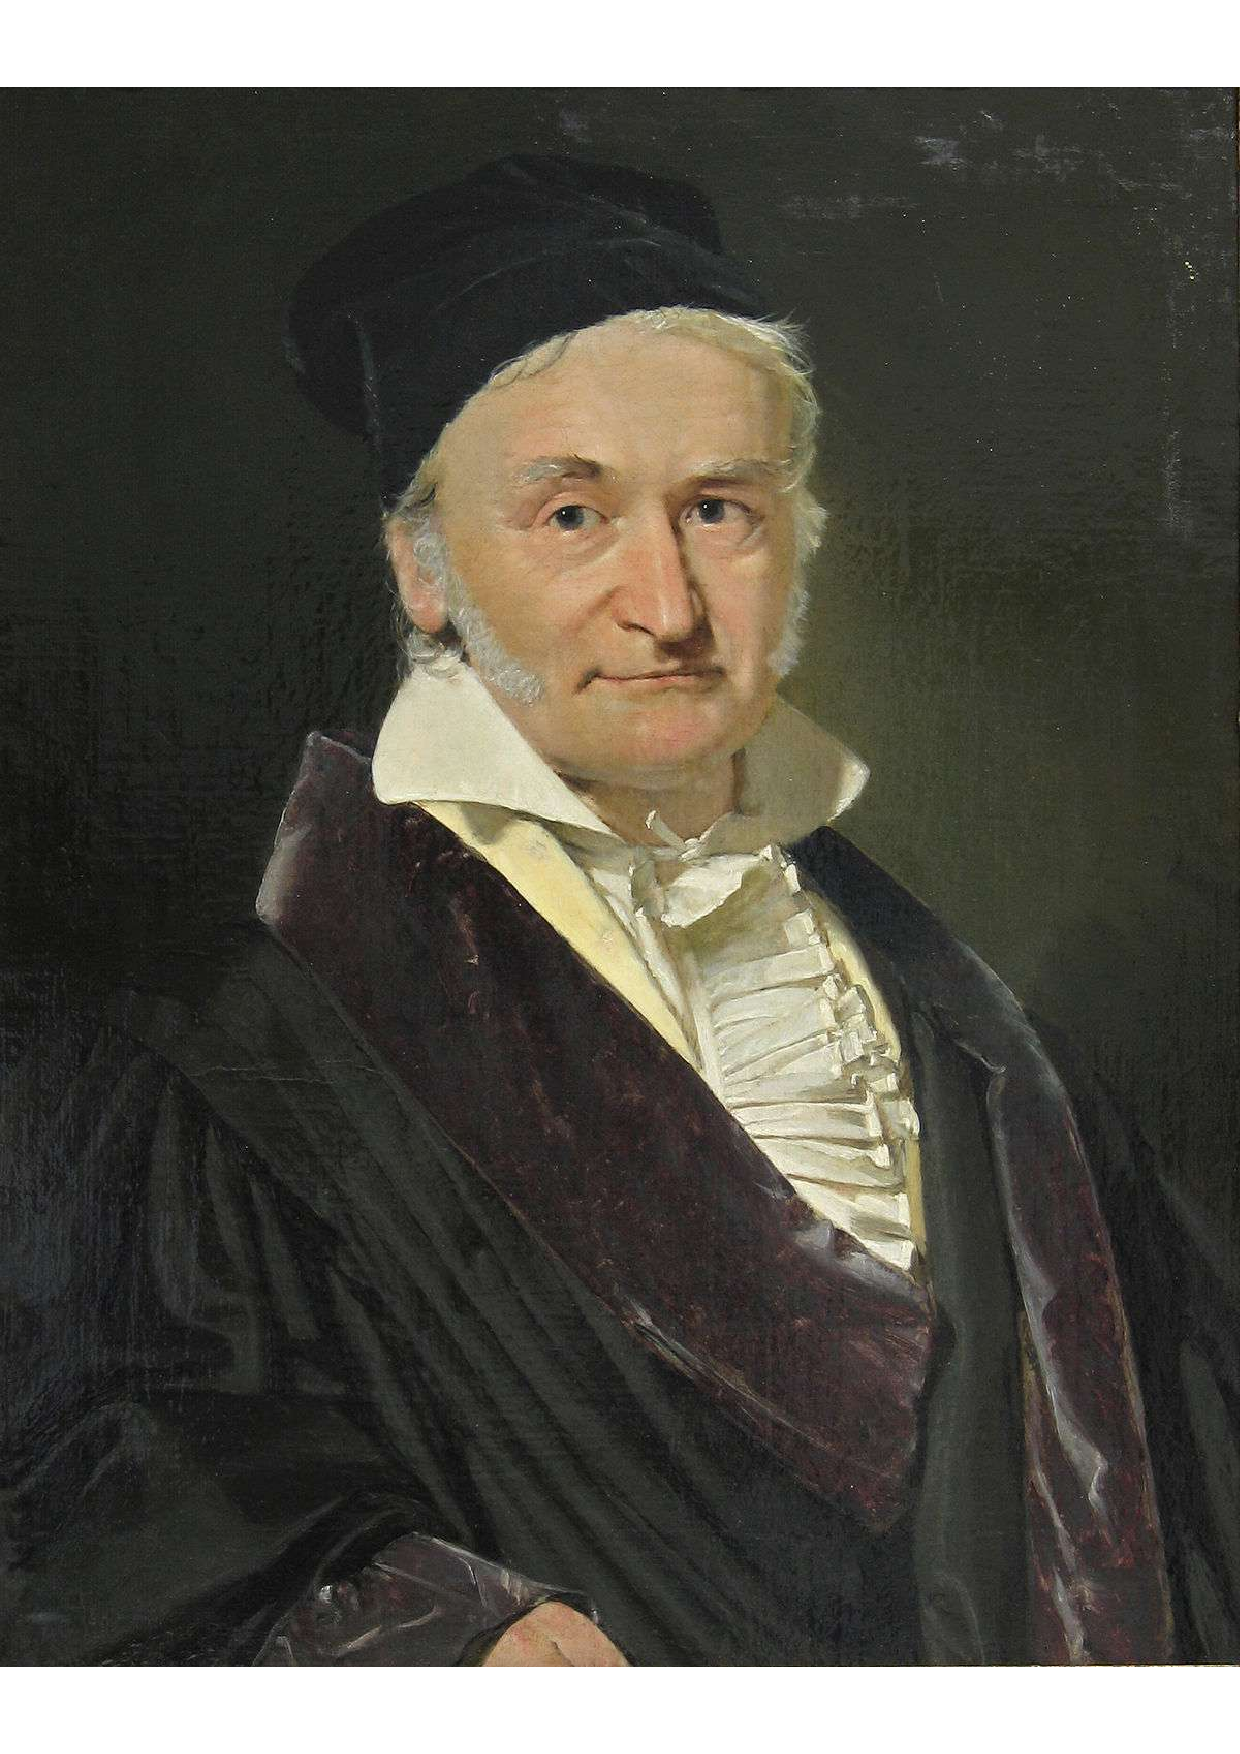
\includegraphics[scale=.20]{Gauss.pdf}
\end{center}
\end{frame}

\begin{frame}{Why Number Theory?}
\begin{stepitemize}
    \item Classical Cryptography built on Number Theory.
    \item Some modern cryptographic schemes(Diffie-Helman, RSA) depend on basic Number Theoretic tools.
    \item Number theoretic tools (Fermat's Little Theorem, Euler's Totient Function, congruences, etc.) appear heavily in homomorphic encryption
    \item Foundation for subsequent topics (Groups, Rings and Fields) to fully understand HE.
\end{stepitemize}
\end{frame}

\begin{frame}

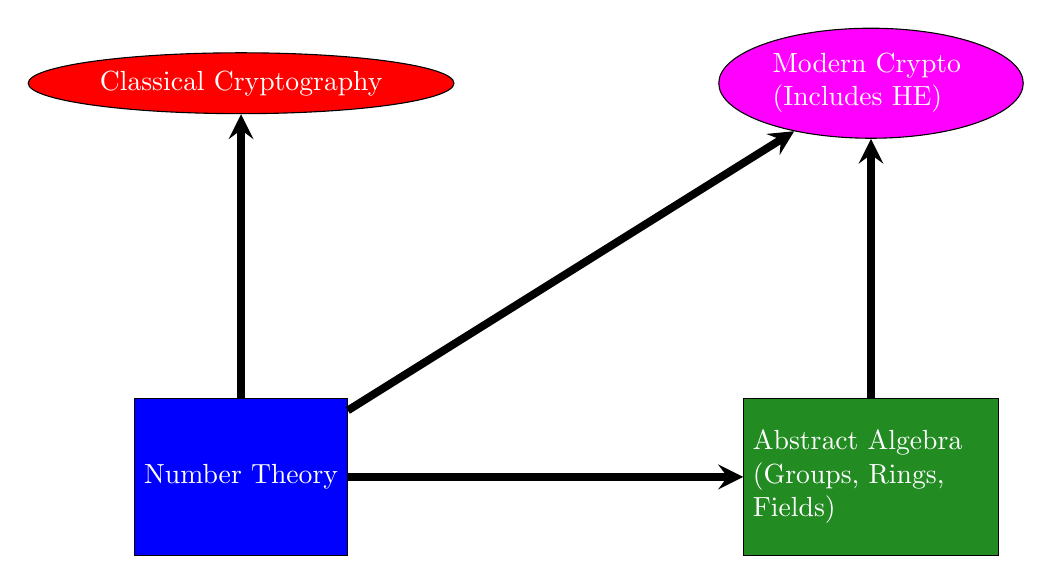
\begin{tikzpicture}
 \node[fill=red, text=white, ellipse,draw] (e1) at (0,5) {Classical Cryptography};
\node[fill=Fuchsia, text=white, ellipse,draw, text width=2.5cm] (e2) at (8,5) {Modern Crypto (Includes HE)};
    \node[fill=blue, text=white, rectangle,draw,  minimum width = 2cm,
    minimum height = 2cm] (r1) at (0,0) {Number Theory};


 \node[fill=ForestGreen, text=white, rectangle,draw,  minimum width = 2cm,
    minimum height = 2cm, text width=3cm] (r2) at (8,0) {Abstract Algebra
    (Groups, Rings, Fields)};

\draw [-stealth, line width=1mm] (r1)--(e1);
\draw [-stealth, line width=1mm] (r1)--(e2);
\draw [-stealth, line width=1mm] (r1)--(r2);
\draw [-stealth, line width=1mm] (r2)--(e2);
%\draw (X)--(P1);
%\draw (X)--(P2);
%\draw (X)--(Pk)
\end{tikzpicture}

\end{frame}


\section{Division Algorithm}

\begin{frame}{Division Algorithm}
\begin{stepitemize}
    \item Basis of congruences.
    \item Main idea: if $a,b \in \Z$ with $b\neq 0$,
    $$a=bq+r, \:\:\:\: 0\leq r <|b|.$$
    \item (As is done in HE), other intervals can be chosen
    \item Dividing by 23, possible intervals:
    $$[0,22], \:\:\:\:\:\: [-11,11], \:\:\:\:\:\: [3,25], \dots $$
\end{stepitemize}
\end{frame}

\begin{frame}
\begin{stepitemize}
\item[]
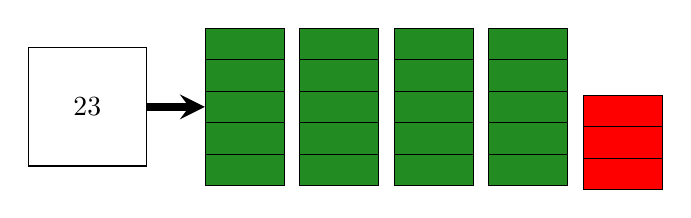
\begin{tikzpicture}
\node[rectangle, draw,  minimum width = 1.5cm,
    minimum height = 1.5 cm](r) at (-2,0){23};
\tikzset{every node/.style={rectangle split,
        rectangle split parts=5, draw, minimum width=1cm}}
  \node[rectangle split part fill={ForestGreen}] (s)at (0,0) {};
  \node[rectangle split part fill={ForestGreen}] at (1.2,0) {};
  \node[rectangle split part fill={ForestGreen}]          at (2.4,0)  {};
  \node[rectangle split part fill={ForestGreen}]                  at (3.6,0) {};

\tikzset{every node/.style={rectangle split,
        rectangle split parts=3, draw, minimum width=1cm}}

\node[rectangle split part fill={red}]  at (4.8,-0.45) {};
\draw [-stealth, line width=1mm] (r)--(s);
\end{tikzpicture}

\bigskip
\item So $23=5\cdot 4+3$.
\item If we use the interval $[-2,2]$ for example.
\item In that case we would have $23=5\cdot 5-2.$
\item {\bf Exercise:} In the following divide $a$ by $b$ with the remainder in the given interval:
$$a=134, \:\: b=23,\:\:\: [-11,11]$$
$$a=245, \:\: b=11, \:\:\: [5, 15]$$
$$a=135, \:\: b=21, \:\:\: [-13, 7]$$

\end{stepitemize}
\end{frame}

\begin{frame}{Some Consequences}
\begin{stepitemize}
    \item Every integer is of the form $3k, 3k+1, 3k+2$
    \item $x^2$ is of the form $4k$ or $4k+1$ for any integer $x$.
    \item If $x$ is odd, then $x^2+1$ is of the form $8k+1$.
    \item Every prime $>3$ is of the form $6k+1$ or $6k+5$.
\end{stepitemize}
\end{frame}

\section{Divisibility}
\begin{frame}{Divisibility}
\begin{stepitemize}
\item Follows from division algorithm naturally (remainder=0)
\item If $a=bq$ for an integer $q$, then ``$b$ divides $a$" and denote by $b|a$.
\item Divisibility Algebra:
\begin{itemize}
    \item If $a|b$ and $c|d$, then $ac|bd$.
    \item If $a|b$ and $b|c$, then $a|c$.
    \item $a|b$ and $b|a$ if and only if $a=\pm b$
    \item If $a|b$ and $b\neq 0$, then $|a|\leq |b|$.
    \item If $a|b$ and $a|c$, then $a|(bx+cy)$ for all $x,y\in \Z$.
\end{itemize}
\end{stepitemize}
\end{frame}
\begin{frame}

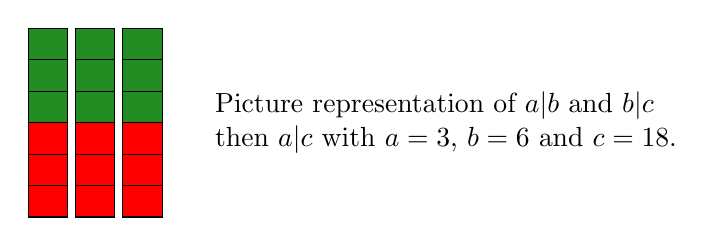
\begin{tikzpicture}
 \node[text width=6cm, anchor=west, right] at (3,0)
    {Picture representation of $a|b$ and $b|c$ then $a|c$ with $a=3$, $b=6$ and $c=18$.};
\tikzset{every node/.style={rectangle split,
        rectangle split parts=6, draw, minimum width=.5cm}}
  \node[rectangle split part fill={ForestGreen, ForestGreen, ForestGreen, red}] (s)at (1,0) {};
  \node[rectangle split part fill={ForestGreen, ForestGreen, ForestGreen, red}] at (1.6,0) {};
  \node[rectangle split part fill={ForestGreen, ForestGreen, ForestGreen, red}]          at (2.2,0){};
 \end{tikzpicture}
\end{frame}

\section{GCD}
\begin{frame}{GCD}
\begin{stepitemize}
    \item The GCD of two non-negative ntegers $a, b$ (not both 0) is defined to be $d$ if
    \begin{itemize}
        \item $d|a$ and $d|b$, (so $d$ is a common divisor, the ``CD") and
    \item If $e$ is a positive number such that $e|a$ and $e|b$, then $e\leq d$ (so $d$ is the greatest among common divisors, the ``G").
    \item The previous condition can be replaced by
    ``if $e|a$ and $e|b$ then $e|d$."
    \end{itemize}
\item $(a,a)=a$, $(a,0)=a$ ($a>0$)
\item if $a|b$, then $(a,b)=a$.
\item Instrumental for things like ``multiplicative inverse", ``Euler's congruence", ``multiplicative group mod $n$", etc.

\end{stepitemize}
\end{frame}

\begin{frame}
\begin{stepitemize}
\item If $(a,b)=1$, then $a$ and $b$ are called ``relatively prime" or ``coprime".
\item {\bf Bezout's Theorem:} If $(a,b)=d$, then $d=ax+by$ for some integers $x,y$.
\item {\bf Special case:} $(a,b)=1$ if and only if $ax+by=1$ for some integers $x,y$.
\item {\bf Example:} $(22,30)=2=22\cdot(-4)+30\cdot3$, \:\: $(15,37)=1 = 15\cdot 5+37\cdot(-2)$.
\end{stepitemize}

\end{frame}
\begin{frame}{Examples}
\begin{stepitemize}
\item Let us find $(16,24)$.
\item $A:$ the set of divisors of $16$ and $B$: the set of divisors of $24$.

\bigskip

\item[]

\begin{center}
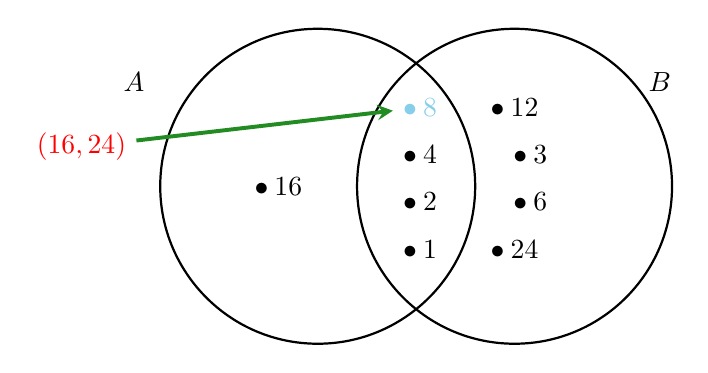
\begin{tikzpicture}[thick,
    set/.style = {circle,
        minimum size = 3cm}]

% Set A
\node[set,label={135:$A$}] (A) at (-1,0) {};

% Set B
\node[set,label={45:$B$}] (B) at (3,0) {};

 \node[text=SkyBlue] (v2) at ( 1.3,1)    {$\bullet \:8$};
 \node at ( 1.3,0.4)    {$\bullet \:4$};
\node at ( 1.3,-0.2)    {$\bullet \: 2$};
\node at ( 1.3,-0.8)    {$\bullet \: 1$};
\node at ( -0.5,0)    {$\bullet \: 16$};
\node at ( 2.7,0.4)    {$\bullet \: 3$};
\node at ( 2.7,-0.2)    {$\bullet \: 6$};
\node at ( 2.5,1)    {$\bullet \: 12$};
\node at ( 2.5,-0.8)    {$\bullet \: 24$};
% Intersection
\node[text=red] (v1) at ( -3,0.5)    {$(16,24)$};
% Circles outline
\draw (0,0) circle(2cm);
\draw (2.5,0) circle(2cm);
\draw [-stealth, ForestGreen, line width=0.5mm](v1)->(v2);
\end{tikzpicture}
\end{center}
\end{stepitemize}

\end{frame}

\begin{frame}{Examples}
\begin{stepitemize}
\item If $(a,b)=1$, $a$ and $b$ have no common factors (other than $1$ of course).
\item For example find $(15,28)$.
\item $C$: set of divisors of $15$ and $D$: set of divisors of $28$.

\bigskip

\item[]
\begin{center}
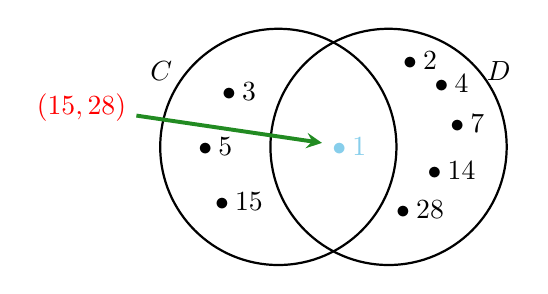
\begin{tikzpicture}[thick,
    set/.style = {circle,
        minimum size = 2cm}]

% Set A
\node[set,label={135:$C$}] (C) at (-0.5,0) {};

% Set B
\node[set,label={45:$D$}] (D) at (1.8,0) {};

 \node[text=SkyBlue] (v2) at ( 0.9,0)    {$\bullet \:1$};
\node at ( -0.5,0.7)    {$\bullet \: 3$};
\node at ( -0.8,0)    {$\bullet \: 5$};
\node at ( 1.8,1.1)    {$\bullet \: 2$};
\node at ( 2.2, 0.8)    {$\bullet \: 4$};
\node at ( 2.4, 0.3)    {$\bullet \: 7$};
\node at ( 2.2,-0.3)    {$\bullet \: 14$};
\node at ( 1.8,-0.8)    {$\bullet \: 28$};
\node at ( -0.5,-0.7)    {$\bullet \: 15$};
% Intersection
\node[text=red] (v1) at ( -2.5,0.5)    {$(15,28)$};
% Circles outline
\draw (0,0) circle(1.5cm);
\draw (1.4,0) circle(1.5cm);
\draw [-stealth, ForestGreen, line width=0.5mm](v1)->(v2);
\end{tikzpicture}
\end{center}
\end{stepitemize}

\end{frame}
\begin{frame}[fragile]{Euclidean Algorithm}
\begin{stepitemize}
    \item Helps us calculate the GCD without the G, C or D.
    \item Depends on the following idea: if $a=bq+r$, then $(a,b)=(r,b)$.
    \item Algorithm: If $b|a$, then $(a,b)=b$, else if $a=bq+r$, then $(a,b)=(b,r)$.
    \item A nice recursive algorithm.
    \item Code snippet assuming ($a\geq b$): \\

     \rule{\textwidth}{1pt}
\begin{minted}{C++}
if (a%b==0) return b;
  else
  return gcd(b,a%b);
\end{minted}
\rule{\textwidth}{1pt}

\item {\bf Example:} $(30,12)=(12,6)=6$,\:\:\: $(a+1,a)=(a,1)=1$.
\end{stepitemize}
\end{frame}

\begin{frame}{Extended Euclidean Algorithm}
\begin{stepitemize}
\item Steps for Euclidean Algorithm can be reversed to find $x,y$ such that $(a,b)=ax+by$.
\item Example: $a=134$, $b=28$
\item \begin{align*}
    134 &=4\cdot 28+22 \:\:\:\:\:\:\:\:\:  ({\color{ForestGreen} (134,28)=(28,22)})\\
    28 &=1\cdot 22+6 \:\:\:\:\:\:\:\:\:\:\:  ({\color{ForestGreen} (28,22)=(22,6)})\\
    22&=3\cdot 6+4  \:\:\:\:\:\:\:\:\:\:\:\:\:  ({\color{ForestGreen}(22,6)=(6,4)})\\
    6&=1\cdot 4+2   \:\:\:\:\:\:\:\:\:\:\:\:\:  ({\color{ForestGreen}(6,4)=(4,2)})\\
    4&=2\cdot 2.
\end{align*}
\item This shows that $(134,28)=2$
\item We can find coefficients $x,y$ by reversing the steps.
\item {\color{ForestGreen}$2$}$=6-4 = 6-(22-3\cdot 6)=4\cdot 6-22 = 4(28-22)-22 = 4\cdot 28-5\cdot 22 = 4\cdot 28-5(134-4\cdot 28)$.
\item $=4\cdot 28-5\cdot 134 +20\cdot 28 = {\color{red}(-5)}\cdot 134+{\color{red} 24}\cdot 28$.
\end{stepitemize}
\end{frame}

\begin{frame}{Exercise}
\begin{stepitemize}
\item For the following pairs of numbers $a,b$ find the GCD using the Euclidean algorithm and find $x,y \in \Z$ such that $(a,b)=ax+by$ using the Extended Euclidean Algorithm
\item $a=245, b=35$
\item $a=432, b=346$
\item $a=1256, b=654$
\end{stepitemize}

\end{frame}

\section{Prime Numbers}
\begin{frame}{Prime Numbers}
    \begin{stepitemize}
        \item Building blocks of all integers
        \item Nice properties leading to cryptographic schemes
        \item Have many uses in groups, fields, etc.
        \item Defined as positive integer greater than 1, that has only two positive divisors: $1$ and itself.
        \item So a prime is irreducible, i.e., cannot be written as a product of two smaller numbers.
        \item $2,3,5,7,11,13, \dots$
        \item $2$ is the only even prime
        \item There are infinitely many of them (Euclid)
        \item No known closed-form function that gives all the primes.
    \end{stepitemize}
\end{frame}

\begin{frame}{A fun exercise}
\begin{stepitemize}
\item {\bf Claim:} $x^2+x+41$ is prime for all integers $x\geq 0$:

\item[]
\scriptsize{
\begin{table}[H]
    \centering
    \begin{tabular}{| c | c |c ||c|c|c|}
    \hline
         $x$ & $x^2+x+41$ & Prime? & $x$ & $x^2+x+41$ & Prime?\\
         \hline
         \hline
         $0$  & $41$ & Y & $20$ &$461$ & Y \\
         \hline
         $1$  & $43$ & Y & $21$ &$503$ & Y \\
         \hline
         $2$ & $47$ & Y & $22$ & $547$ & Y\\
         \hline
         $3$ & $53$ & Y & $23$ & $593$ & Y\\
         \hline
         $4$ & $61$ & Y & $24$ & $641$ & Y\\
         \hline
         $5$ & $71$ & Y & $25$ & $691$ & Y\\
         \hline
          $6$ & $83$ & Y & $26$ & $743$ & Y\\
         \hline
         $\vdots$ & $\vdots$ & $\vdots$ & $\vdots$ & $\vdots$ & $\vdots$\\
         \hline
         $17$ & $347$ & Y & $37$ & $1447$ & Y\\
         \hline
         $18$ & $383$ & Y & $38$ & $1523$ & Y\\
         \hline
         $19$ & $421$ & Y & $39$ & $1601$ & Y\\
         \hline

    \end{tabular}
    \label{tab:my_label}
\end{table}
}
 \item So does this function give primes all the time?
 \item Well, $40^2+40+41=1681=41^2$, so NO!.
 \item More trivially, $41^2+41+41=41(41+1+1)=41\cdot 43$.
 \end{stepitemize}
\end{frame}

\begin{frame}{A Homework Exercise}
    \begin{stepitemize}
    \item Can you find another function like $x^2+x+41$ that gives primes for many consecutive values of $x$?
    \item If you are up for a theoretical side to this
    \item Here is something you can try:
    \item For $x^2+x+a$ to work like above we must have $a\equiv 2$ or $11$ $\pmod{15}$.
    \item Of course this is not sufficient as you can see on examples.
    \end{stepitemize}
\end{frame}

\begin{frame}{More on Primes}
\begin{stepitemize}
\item If $p$ is prime $(a,p)=1$ or $p$ depending on $p\nmid a$ or $p|a$ respectively.
\item ({\bf Euclid's Lemma}) $p>1$ is prime if and only if $p|ab$ implies $p|a$ or $p|b$.
\item More generally, if $p$ is prime, $p|a_1a_2\dots a_k$ implies $p|a_i$ for some $i$.
\item ({\bf Fund. Thm. Arith}) Every integer $>1$ can be written as a product of primes uniquely.
\item So, if $n>1$, then $n=p_1^{\alpha_1}p_2^{\alpha_2}\dots p_k^{\alpha_k}$.
\item For example $360=2^3\cdot 3^2\cdot 5$, $288=2^5\cdot 3^2$.
\end{stepitemize}
\end{frame}

\begin{frame}{Consequences of Fundamental Theorem}
\begin{stepitemize}
\item The GCD, LCM, the number of positive divisors can all be deduced from the prime factorization.
\item If $m,n \geq 0$ have prime factorization:
$$n=p_1^{\alpha_1}p_2^{\alpha_2} \dots p_k^{\alpha_k},$$
$$m=p_1^{\beta_1}p_2^{\beta_2} \dots p_k^{\beta_k}$$
where $\alpha_i, \beta_i \geq 0$. (why did we let them be $\geq 0$?)
\item
Then we can write
$$GCD(m,n) = p_1^{\min(\alpha_1, \beta_1)}\cdot p_2^{\min(\alpha_2, \beta_2)} \cdot \dots \cdot p_k^{\min(\alpha_k, \beta_k)}$$

\item
$$LCM(m,n) = p_1^{\max(\alpha_1, \beta_1)}\cdot p_2^{\max(\alpha_2, \beta_2)} \cdot \dots \cdot p_k^{\max(\alpha_k, \beta_k)}.$$

\item $\tau(n)=(1+\alpha_1)(1+\alpha_2)\dots (1+\alpha_k)$ gives us the formula for the number of distinct positive divisors of $n$.
\end{stepitemize}

\end{frame}

\begin{frame}[fragile]{Sieve of Eratosthenes}
\begin{stepitemize}
\item Depends on the following theorem:
\item If $n>1$ is composite, then there exists a prime number $p$ such that $p\leq \sqrt{n}$ and $p|n$.
\item So, if $n>1$ is NOT divisible by any of the primes $\leq \sqrt{n}$, then $n$ must be prime.
\item The following is a code snippet for a primitive primality test using this idea:

\item[] \rule{\textwidth}{1pt}
\begin{minted}{C++}
bool isprime(int n){

  for (int i=2;i*i<=n;i++){
     if (n%i==0)
        return false;
   }
  return true;
}
\end{minted}
\rule{\textwidth}{1pt}
\end{stepitemize}
%\item So, to find all primes from $2$ to $100$, we just need to eliminate multiples of $2,3,5,7$:
%\item[]
 %   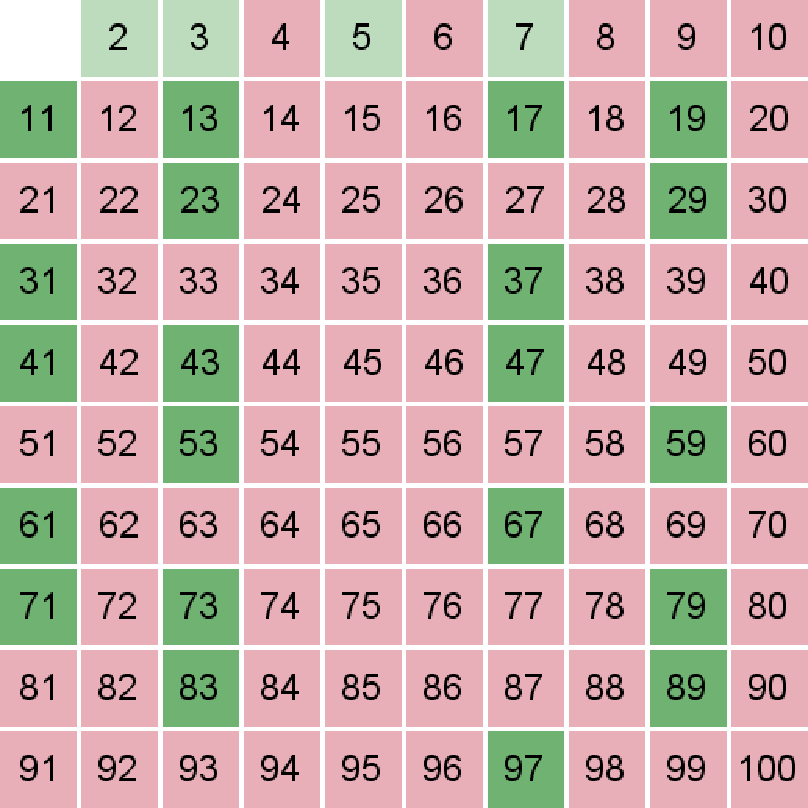
\includegraphics[scale=.30]{Erat.pdf}

%\end{stepitemize}
\end{frame}

\begin{frame}{Finding all primes up to a number}
\begin{stepitemize}
\item Another consequence: to find all primes from $2$ to $100$, we just need to eliminate multiples of $2,3,5,7$. ($\sqrt{100}=10$)
\item This is also known as the Sieve of Eratosthenes:

\bigskip

\begin{center}
    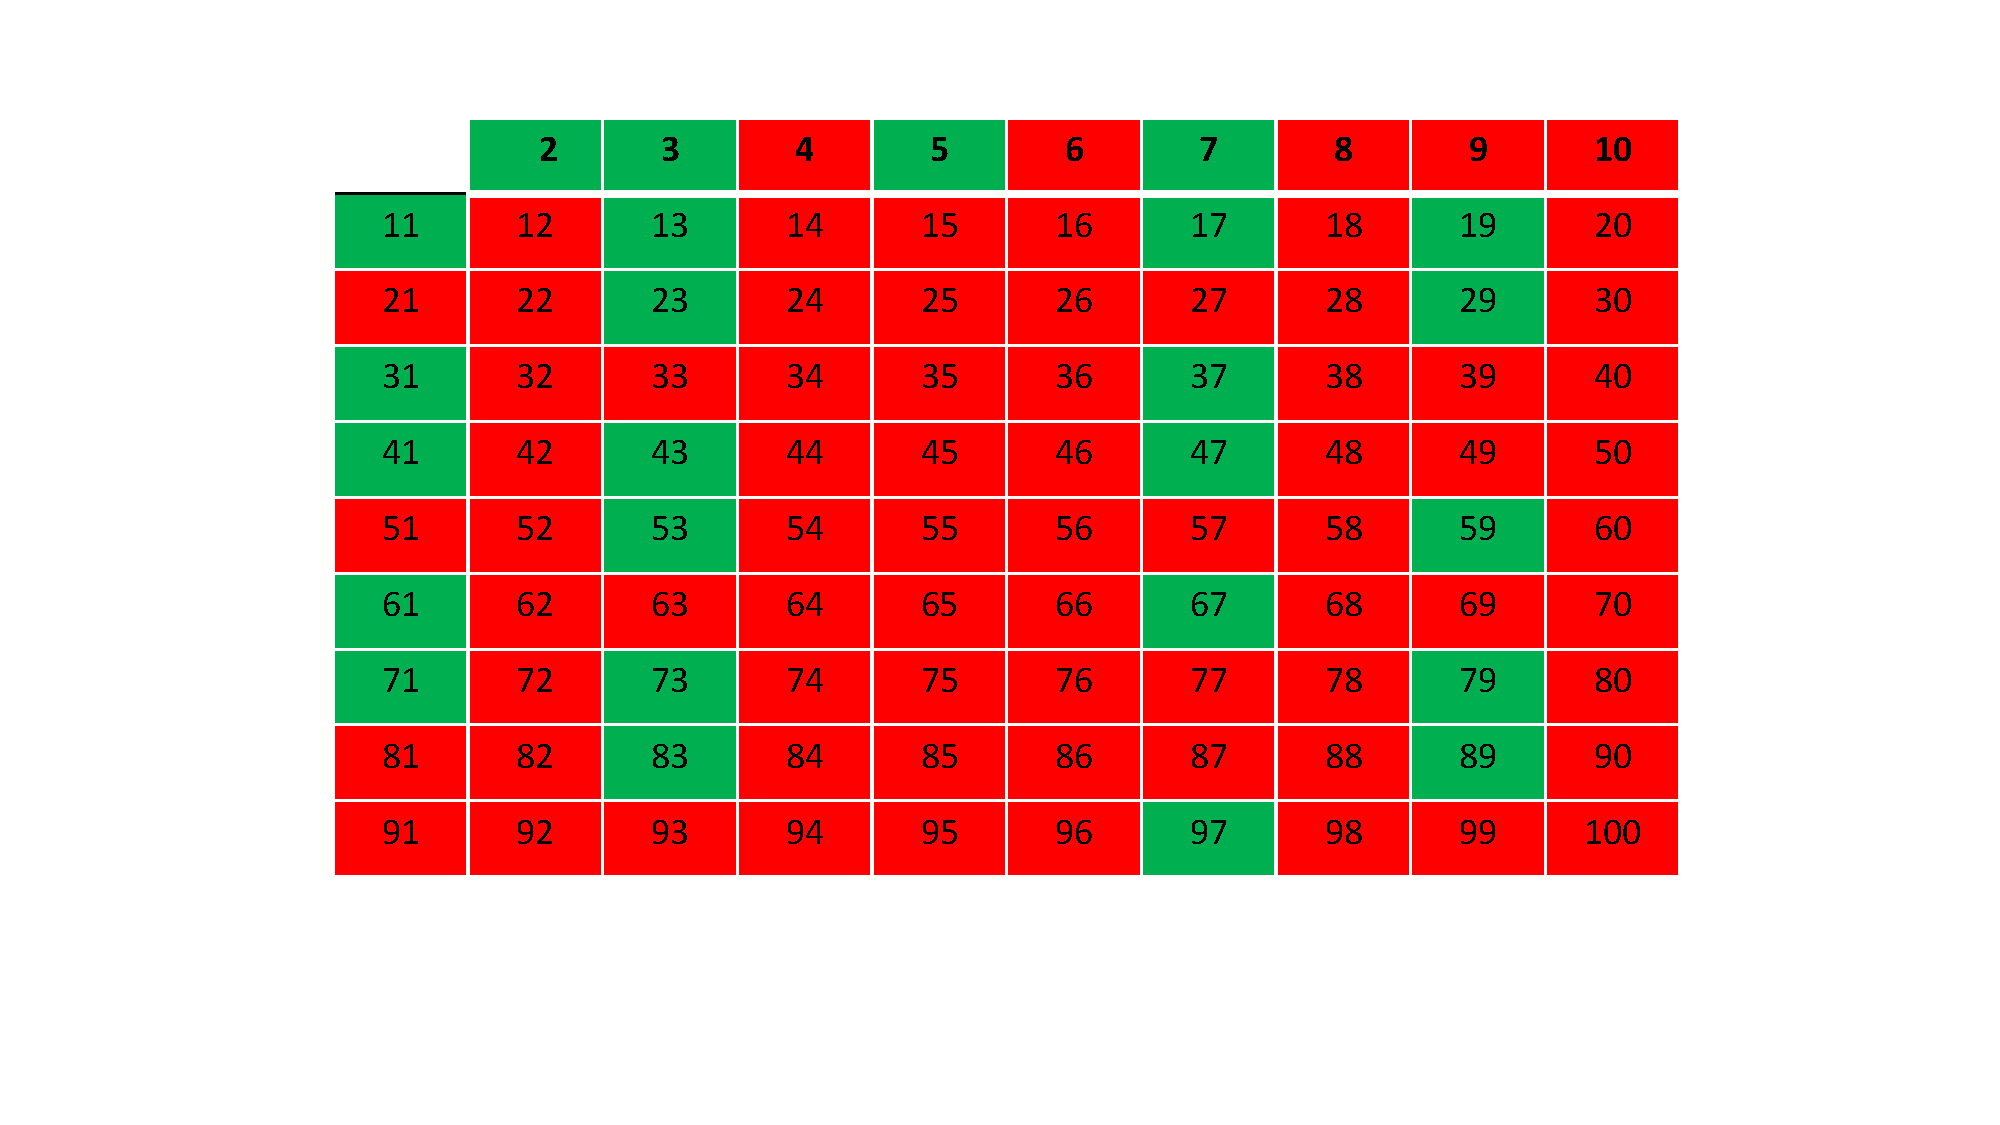
\includegraphics[scale=.40]{erat.pdf}
\end{center}

\end{stepitemize}
\end{frame}

\begin{frame}{Exercises using the theorem}
\begin{stepitemize}
\item Using the theorem try to determine if the following are prime by hand:
\item $541$
\item $257$
\item $843$
\item $1003$.
\item Do you remember divisibility rules for $3,5,7,11$?
\end{stepitemize}

\end{frame}

\section{Congruences}
\begin{frame}{Congruences}
\begin{stepitemize}
\item Directly follows from the Division Algorithm
\item For $m>1$ we say $a\equiv b \pmod{m}$ if $a$ and $b$ leave the same remainder upon dividing by $m$.
\item i.e. $a\equiv b \pmod{m}$ if and only if $m|(a-b)$, or equivalently $a=b+mk$ for some $k$.
\item classical visual for modulo $12$:
    \begin{center}
    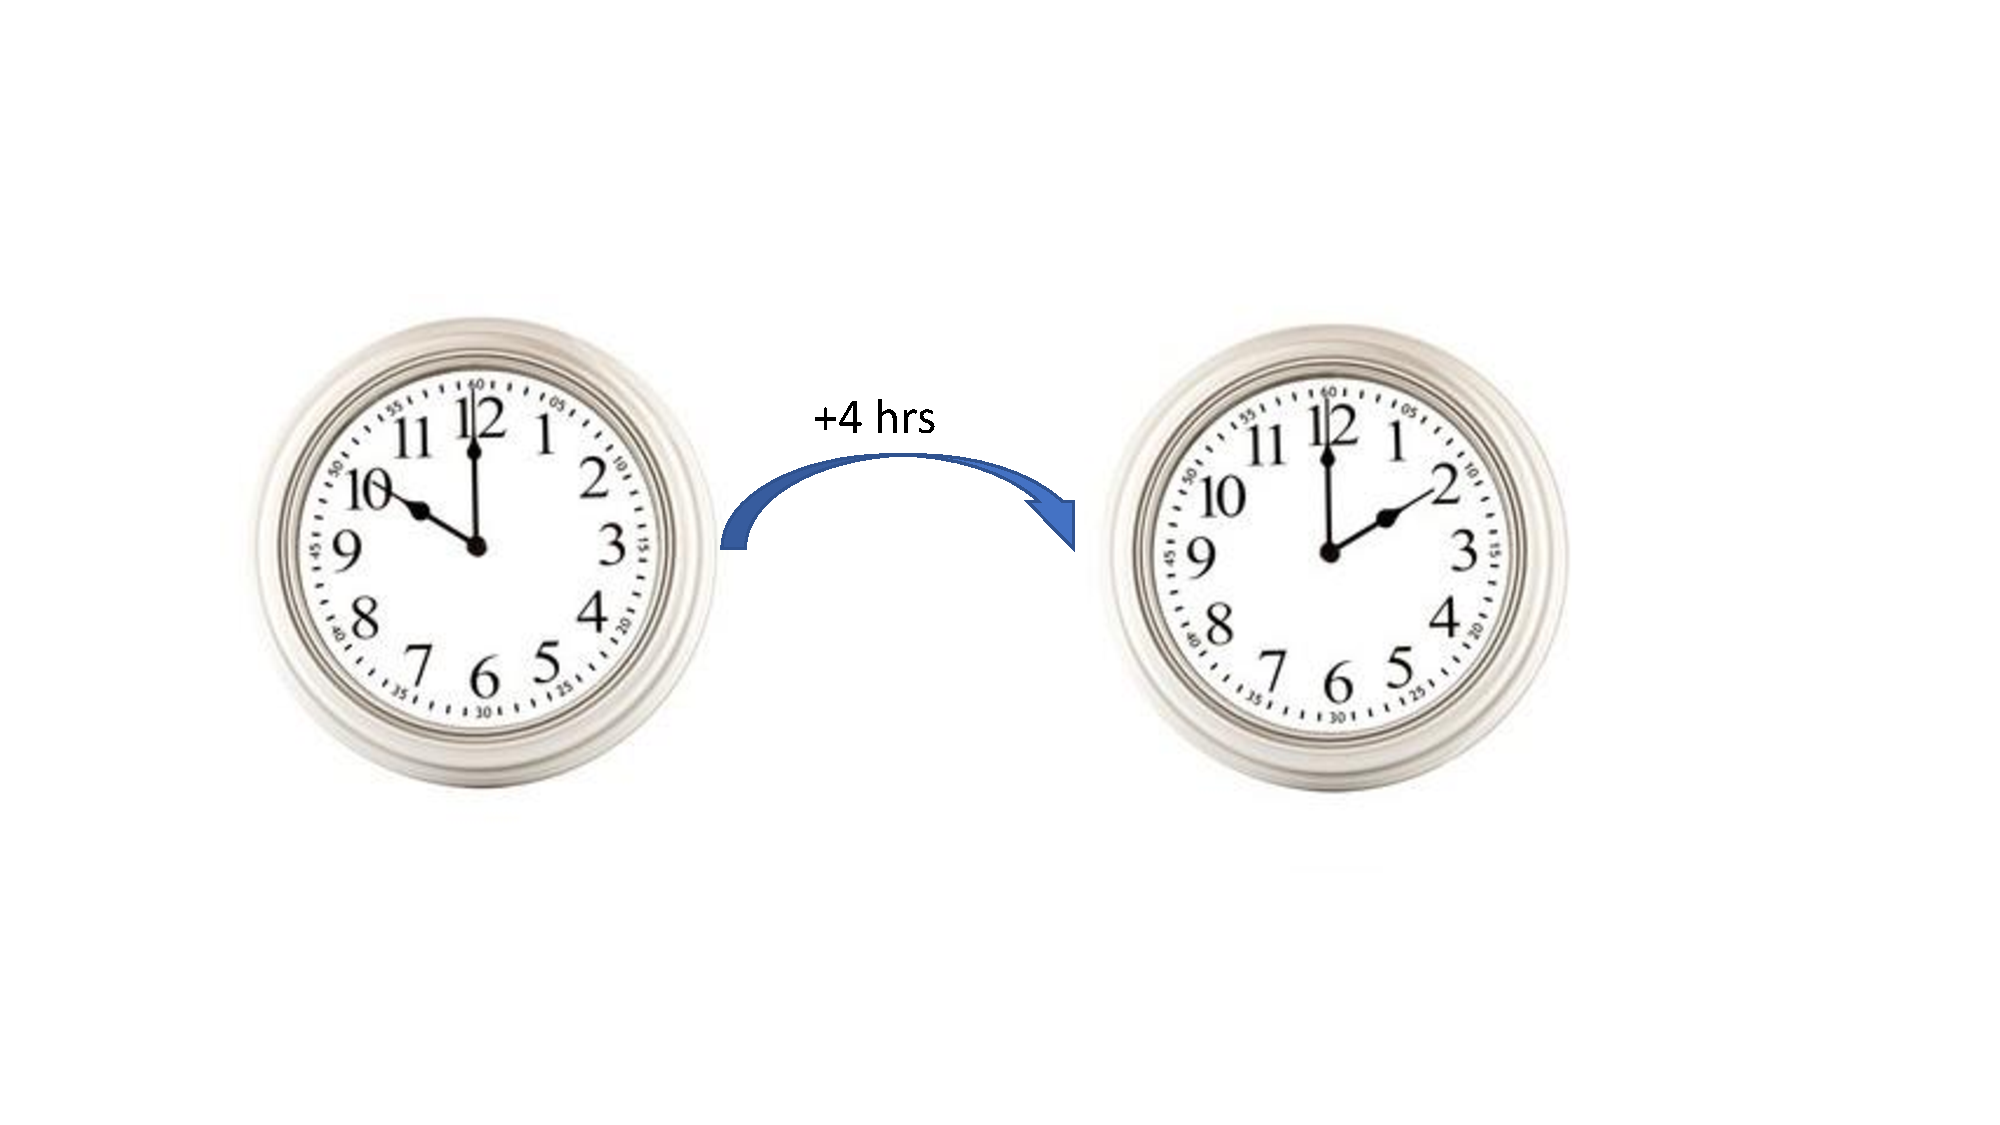
\includegraphics[scale=.35]{clock1.pdf}
\end{center}

\end{stepitemize}
\end{frame}

\begin{frame}{Algebra of Congruences}
\begin{stepitemize}

\item[]{\bf Theorem:}\\
Let $n>1$ be an integer and $a, b, c, d$ be any integers. Then

\begin{enumerate}
    \item $a\equiv a \pmod{n}$.
    \item If $a\equiv b \pmod{n}$, then $b\equiv a \pmod{n}$.
    \item If $a\equiv b \pmod{n}$ and $b\equiv c \pmod{n}$, then $a\equiv c \pmod{n}$.
    \item If $a\equiv b \pmod{n}$ and $c\equiv d \pmod{n}$, then $a+c\equiv b+d \pmod{n}$ and $ac\equiv bd \pmod{n}$.
    \item If $a\equiv b \pmod{n}$, then $a+c\equiv b+c \pmod{n}$ and $ac\equiv bc \pmod{n}$ for all $c\in \Z$.
    \item If $a\equiv b \pmod{n}$, then $a^k \equiv b^k \pmod{n}$ for all positive integers $k$.
\end{enumerate}

\medskip
\item {\bf Remark:}
    \item Properties (1)-(3) imply congruence is an equivalence relation
    \item Property (4) gives us a hint for ``homomorphic encryption".
\end{stepitemize}
\end{frame}

\begin{frame}{Special Congruences: Fermat's Little Theorem}
\begin{stepitemize}
\item If $p$ is a prime number and $p\nmid a$, then we have $a^{p-1} \equiv 1 \pmod{p}$.
\item Another version: if $p$ is prime, then $a^p\equiv a \pmod{p}$ for all integers $a$.
\item To reduce $2^{1798}$ modulo $11$,
$$2^{1798} = (2^{10})^{179}\cdot 2^8 \equiv 2^8=256\equiv 3 \pmod{11}. $$
\item[]     \begin{center}
    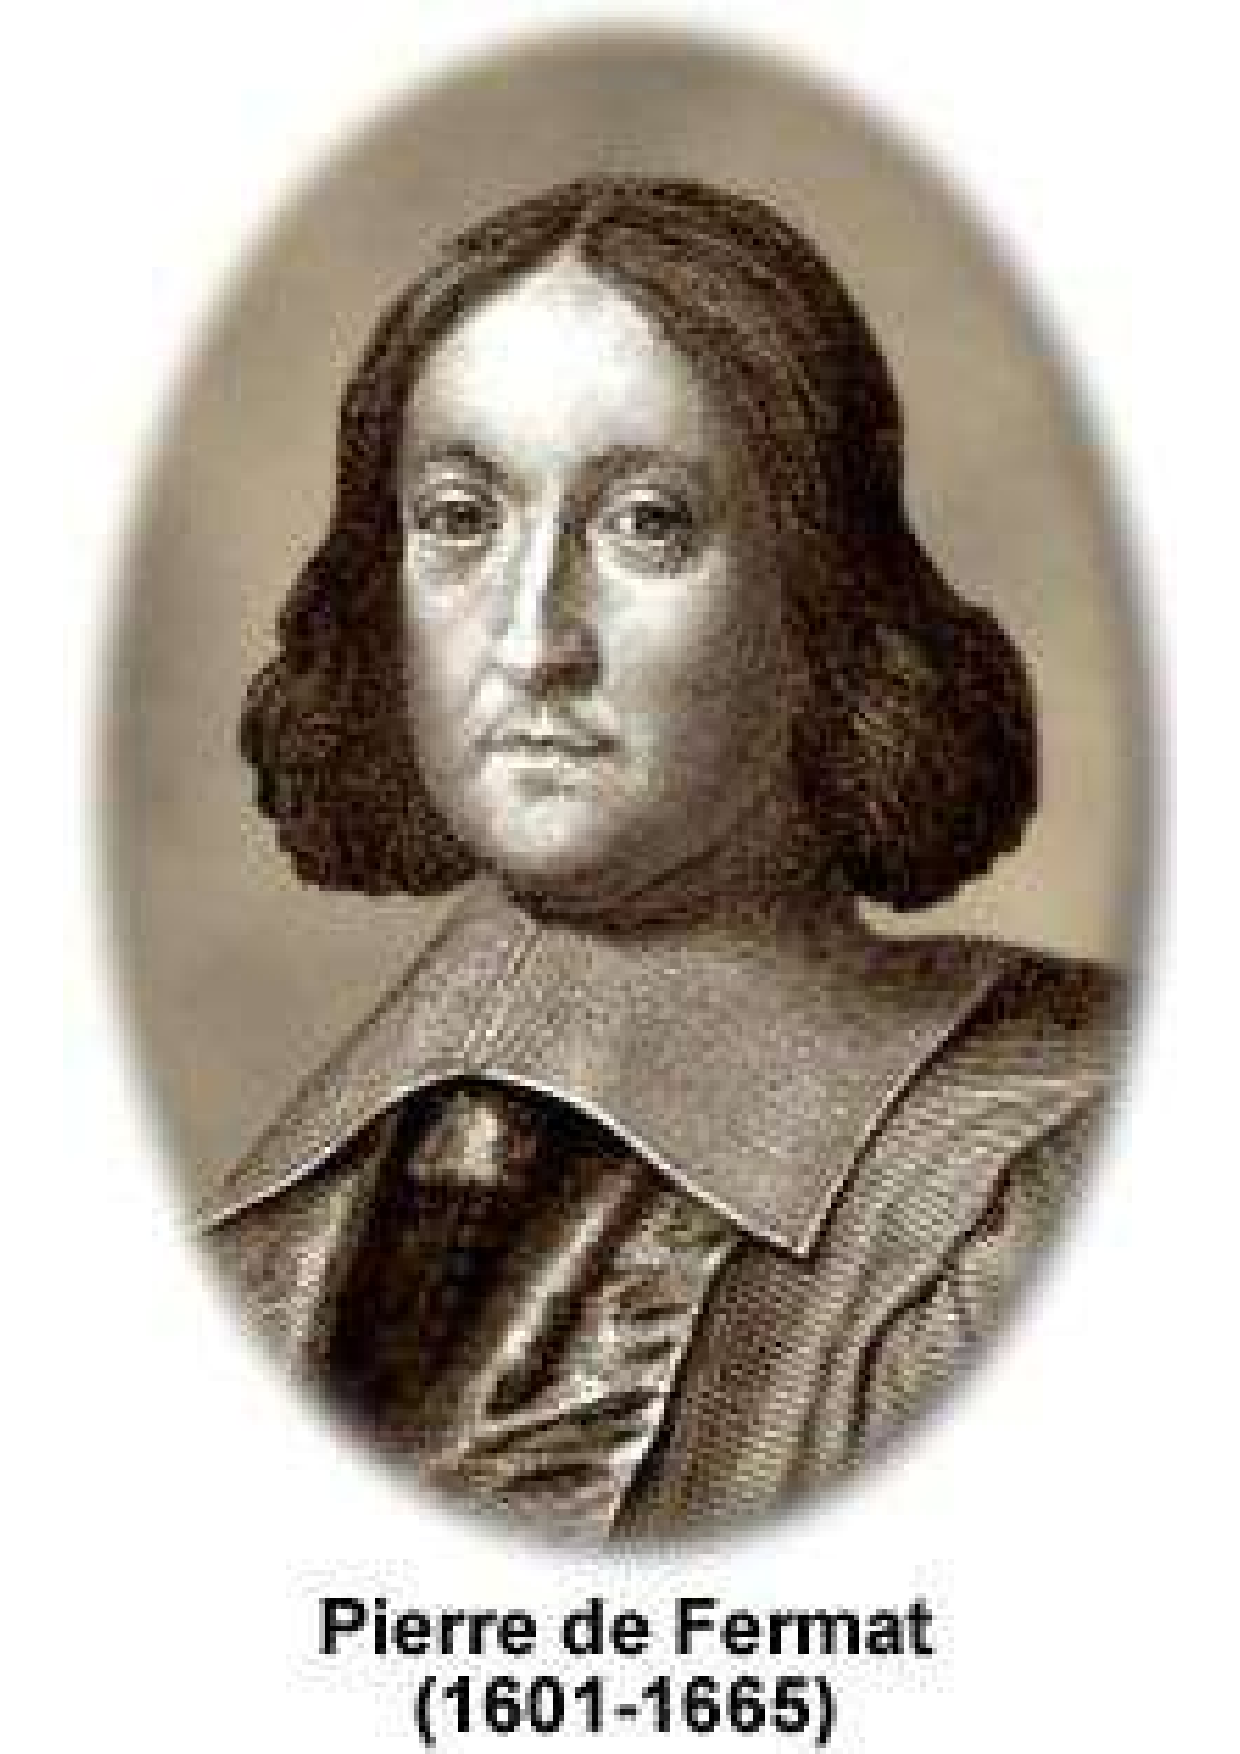
\includegraphics[scale=.180]{fermat.pdf}
\end{center}

\end{stepitemize}
\end{frame}

\begin{frame}{Exercises}
\begin{stepitemize}
\item Using Fermat's congruence reduce the following modulo the corresponding modulus:
\item $342^{1234} \pmod{5}$
\item $23^{254} \pmod{13}$
\item $17^{13}+13^{17} \pmod{7}$

\end{stepitemize}

\end{frame}

\begin{frame}{Special Congruences: Linear Congruences}
\begin{stepitemize}
\item Analogous to linear equations
\item Want to solve $ax\equiv b\pmod{n}$ when $n>1$.
\item Two questions:
\item {\bf {\color{red} 1}}. When are there solutions?
\item {\bf {\color{red} 2}}. If there are solutions how many are there?
\end{stepitemize}
\end{frame}

\begin{frame}{An Example}
\begin{stepitemize}
\item As an example consider the following congruences:
\item $2x\equiv 4 \pmod{8}$.
\item This has two solutions: $2, 6$.
\item $4x\equiv 0 \pmod{8}$.
\item This has four solutions: $0,2,4,6$.
\item $2x\equiv 3 \pmod{8}$.
\item This has no solutions since $2x=3+8k$ implies even=odd.
\item $3x\equiv 5 \pmod{8}$.
\item This has a unique solution. $x=7$.
\item Question: What determines that there are solutions and how can we tell the number of solutions?
\end{stepitemize}
\end{frame}

\begin{frame}{Linear Congruences cont'd}
\begin{stepitemize}
\item {\bf Theorem:} \\
The congruence $ax\equiv b \pmod{n}$ has solutions if and only if $(a,n)|b$. Moreover, if $d=(a,n)$, then the congruence has exactly $d$ incongruent solutions.

\item In particular, if $GCD(a,n)=1$, then $ax\equiv b \pmod{n}$ has a unique solution modulo $n$ for every integer $b$.
\item Consider $9x\equiv 21 \pmod{30}.$

\item We first cancel $3$, which leads to $3x\equiv 7 \pmod{10}$.
\item Multiplying both sides by $7$, we get $x\equiv 9 \pmod{10}$.
\item Then the three solutions are given by $9, 9+10=19, 9+20=29$.
\item Exercise: Solve the congruences
$$18x\equiv 6 \pmod{24}, \:\:\:\: 23x\equiv 4 \pmod{17}.$$
\end{stepitemize}
\end{frame}

\begin{frame}{A Special Case: Multiplicative Inverse}
\begin{stepitemize}
\item For $n>1$ and $a$ an integer, we say $x$ is a multiplicative inverse of $a$ modulo $n$ if $ax\equiv  1 \pmod{n}$.
\item So, by the previous theorem, $a$ has mult. inverse modulo $n$ if and only if $(a,n)=1$.
\item One way to find mult. inverse: Extended Euclidean Algorithm.
\item For example: $(22,35)=1$ and we have $8\cdot 22 +(-5)\cdot 35=1$.
\item Reducing the equation modulo $35$, we see that $22\cdot 8 \equiv 1 \pmod{35}$
\item So the multiplicative inverse of $22$ modulo $35$ is $8$.
\item Exercise: Find the mult. inverse of $232$ modulo $351$, using EEA.
\end{stepitemize}

\end{frame}
\begin{frame}{Special Congruences: Chinese Remainder Theorem(CRT)}
\begin{stepitemize}
\item A powerful tool to solve systems of congruences
\item Can be generalized to rings as well.
\item Has profound impact on applications of HE by constructing slots.

\medskip
\item[]
\begin{center}
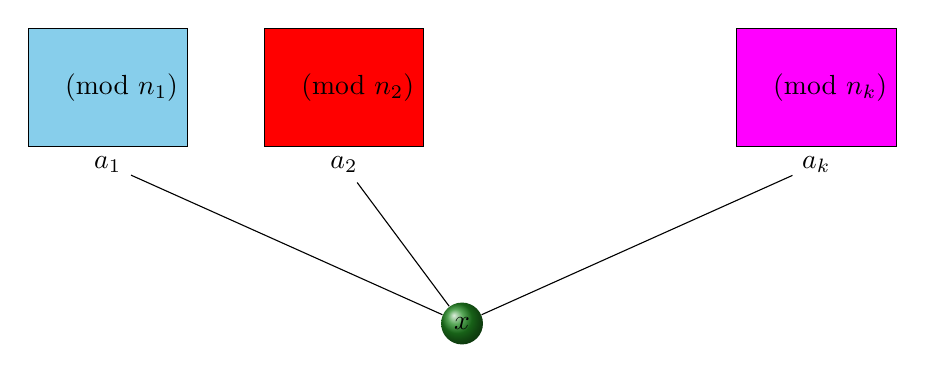
\begin{tikzpicture}
\tikzstyle{point2}=[ball color=ForestGreen, circle, inner sep=0.1cm]

    \node[rectangle,draw, fill=SkyBlue, minimum width = 1.5cm,
    minimum height = 1.5cm] (r1) at (0,0) {$\pmod{n_1}$};

\node [below] (P1) at (r1.south) {$a_1$};

 \node[rectangle,draw, fill=red, minimum width = 1.5cm,
    minimum height = 1.5cm] (r2) at (3,0) {$\pmod{n_2}$};
\node [below] (P2) at (r2.south) {$a_2$};

\filldraw[white] (4.5,0) circle (2pt);

\filldraw[white] (6,0) circle (2pt);

\filldraw[white] (7.5,0) circle (2pt);
 \node[rectangle,draw, fill=Fuchsia, minimum width = 1.5cm,
    minimum height = 1.5cm] (rk) at (9,0) {$\pmod{n_k}$};

\node [below](Pk) at (rk.south) {$a_k$};

\node (X) at (4.5,-3) [point2, text=black] {$x$};
\draw (X)--(P1);
\draw (X)--(P2);
\draw (X)--(Pk);
\end{tikzpicture}
\end{center}
\end{stepitemize}
\end{frame}

\begin{frame}{CRT cont'd}
    \begin{stepitemize}
    \item The main setup is the following:
    \begin{align*}
    x &\equiv a_1 \pmod{n_1} \\
    x &\equiv a_2 \pmod{n_2} \\
    &.\\
    &.\\
    &.\\
    x &\equiv a_k \pmod{n_k}
\end{align*}
\item If $(n_i,n_j)=1$ for all $i,j$ with $i\neq j$, then there is a unique solution to the system modulo $n_1n_2\dots n_k$
\item The solution is given by $$x=a_1N_1N_1^{-1}+a_2N_2N_2^{-1}+\dots +a_kN_kN_k^{-1},$$ where $N_i=\frac{n_1n_2\dots n_k}{n_i}$ and $N_i^{-1}$ is the multiplicative inverse of $N_i$ modulo $n_i$.
    \end{stepitemize}
\end{frame}

\begin{frame}{CRT cont'd}
\begin{stepitemize}
    \item Consider \begin{align*}
    x &\equiv 2 \pmod{3} \\
    x &\equiv 1 \pmod{5} \\
    x &\equiv 3 \pmod{7}.
    \end{align*}
    \item $N_1=5\cdot 7=35$, $N_2=3\cdot 7=21$, $N_3=3\cdot 5=15$.
$N_1^{-1}=2$ modulo $3$, $N_2^{-1}=1$ modulo $5$ and $N_3^{-1} = 1$ modulo $7$. Then
$$x = 2\cdot 35\cdot 2+1\cdot 21\cdot 1+3\cdot 15\cdot 1 = 206 \equiv 101 \pmod{105}.$$
\item[]
\begin{center}
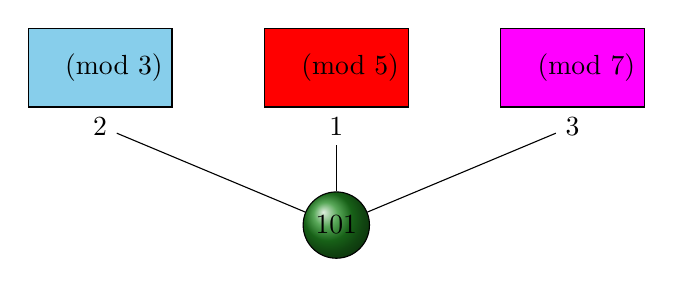
\begin{tikzpicture}
\tikzstyle{point2}=[ball color=ForestGreen, circle, draw=black, inner sep=0.1cm]

    \node[rectangle,draw, fill=SkyBlue, minimum width = 1cm,
    minimum height = 1cm] (r1) at (0,0) {$\pmod{3}$};

\node [below] (P1) at (r1.south) {$2$};

 \node[rectangle,draw,  fill=red, minimum width = 1cm,
    minimum height = 1cm] (r2) at (3,0) {$\pmod{5}$};
\node [below] (P2) at (r2.south) {$1$};
 \node[rectangle,draw,  fill = Fuchsia, minimum width = 1cm,
    minimum height = 1cm] (rk) at (6,0) {$\pmod{7}$};

\node [below](Pk) at (rk.south) {$3$};

\node (X) at (3,-2) [point2, text=black] {$101$};
\draw (X)--(P1);
\draw (X)--(P2);
\draw (X)--(Pk);
\end{tikzpicture}
\end{center}
\end{stepitemize}
    \end{frame}

\begin{frame}{An Alternative Method}
\begin{stepitemize}

\item There is an alternative way to solve the previous system of congruences.
\item Start from the first congruence: $x\equiv 2\pmod{3}$
\item We can write the solution as $x=2+3k$.
\item Now put this into the second congruence
\item $2+3k\equiv 1 \pmod{5}$ , which is equivalent to $3k\equiv 4 \pmod{5}$ and so $k\equiv 3 \pmod{5}$.
\item So we can write $k=3+5m$, which means $x=2+3k=2+3(3+5m)=11+15m$.
\item Put this into the last congruence.
\item $11+15m\equiv 3 \pmod{7}$ or that $m\equiv 6 \pmod{7}$ or that $m=6+7t$.
\item Finally, substitute into $x$:
$$x=11+15m=11+15(6+7t)=101+105t.$$
\end{stepitemize}

\end{frame}

\begin{frame}{Exercise}
\begin{stepitemize}
\item Solve the following system using CRT:
\item \begin{align*}
    x &\equiv 2 \pmod{4} \\
    x &\equiv 3 \pmod{7} \\
    x &\equiv 1 \pmod{9}.
    \end{align*}
\end{stepitemize}

\end{frame}
\section{Euler's Contributions}
\begin{frame}{Euler's Totient Function}
\begin{stepitemize}
    \item for a positive integer $n$, $\phi(n)$ counts the number of $x\leq n$ such that $(x,n)=1$.
    \item We call $\Z_n^{*} = \{1\leq x\leq n| (x,n)=1\}$ the ``Complete Set of Reduced Residue Classes"(CSRRC). (So $\phi(n)=|\Z_n^{*}|$.)
    \item Why do we need them?
    \item Because an element $a$ has a multiplicative inverse mod $n$ if and only if $(a,n)=1$.
    \item[]     \begin{center}
    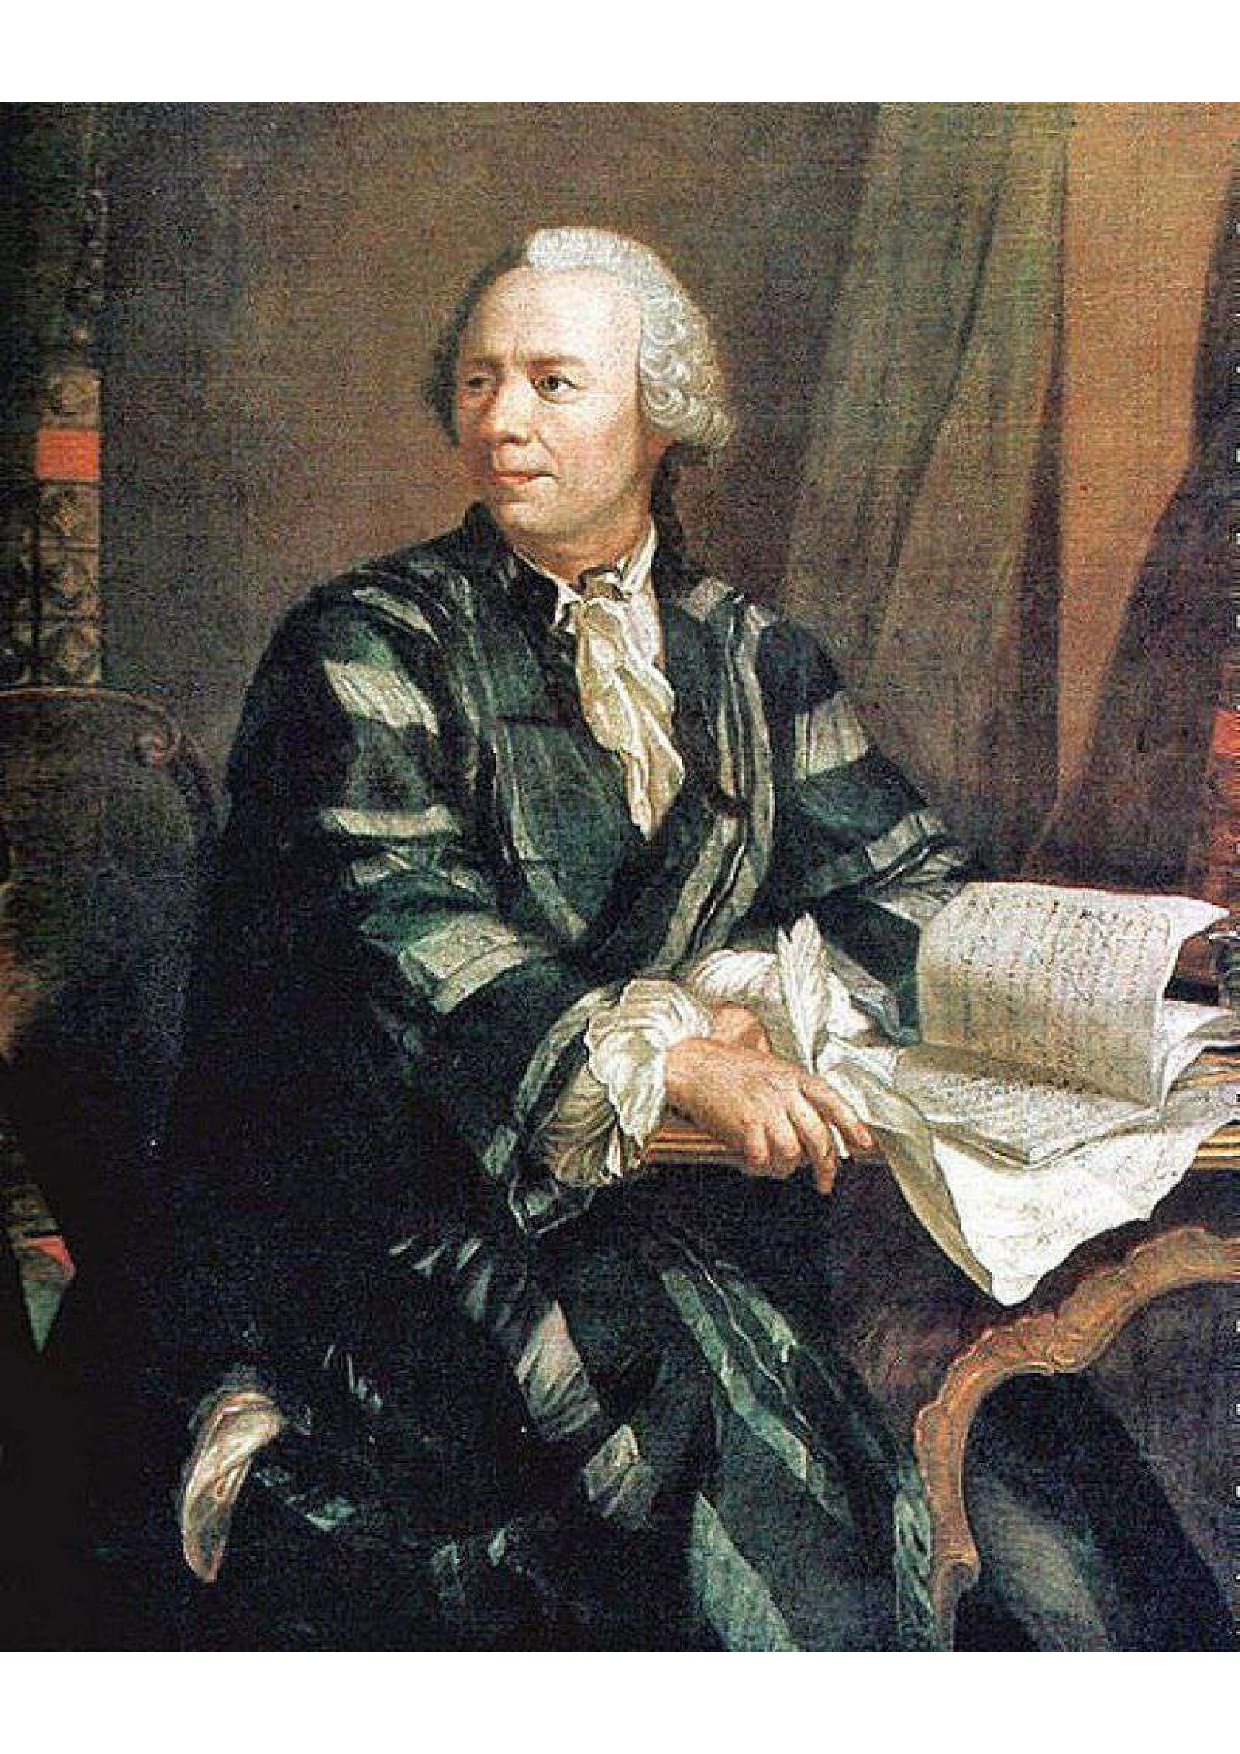
\includegraphics[scale=.170]{Leonhard-Euler.pdf}
\end{center}

\end{stepitemize}

\end{frame}

\begin{frame}{Euler's Totient Continued}
\begin{stepitemize}
    \item For example, $\phi(1)=\phi(2)=1$, $\phi(3)=\phi(4)=\phi(6)=2$, $\phi(5)=4$, etc.
    \item Clearly $\phi(p)=p-1$ if $p$ is prime. (Why?)
    \item $\phi(p^n)=p^n-p^{n-1} = (p-1)p^{n-1}$, because we just take away from the set $\{1,2,3, \dots, p^n\}$ all multiples of $p$, which are just
    $$p\cdot 1, p\cdot 2, \dots, p\cdot p^{n-1}.$$
    \item To find a general formula we need an important result.
    \item $\phi$ is multiplicative.
    \item That is if $(m,n)=1$, then $\phi(mn)=\phi(m)\phi(n)$.
\end{stepitemize}
\end{frame}
\begin{frame}{Multiplicative Totient}
The following picture shows the multiplicative nature of the Totient function.

\bigskip

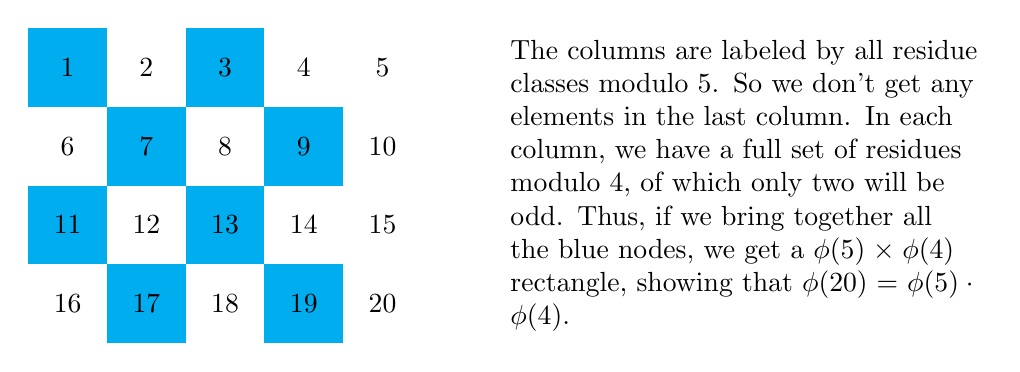
\begin{tikzpicture}
\node[text width=6cm, anchor=west, right] at (6,2)
    {The columns are labeled by all residue classes modulo $5$. So we don't get any elements in the last column. In each column, we have a full set of residues modulo $4$, of which only two will be odd. Thus, if we bring together all the blue nodes, we get a $\phi(5) \times \phi(4)$ rectangle, showing that $\phi(20)=\phi(5)\cdot \phi(4)$.};

\draw[step=1cm,white] (0,0) grid (5,4);
\draw (0.5,3.5) node[fill=cyan, text=black, rectangle, minimum width = 1cm, minimum height = 1cm]{1};
\draw (1.5,3.5) node{2};
\draw (2.5,3.5) node[fill=cyan, text=black, rectangle, minimum width = 1cm, minimum height = 1cm]{3};
\draw (3.5,3.5) node{4};
\draw (4.5,3.5) node{5};
\draw (0.5,2.5) node{6};
\draw (1.5,2.5) node[fill=cyan, text=black, rectangle, minimum width = 1cm, minimum height = 1cm]{7};
\draw (2.5,2.5) node{8};
\draw (3.5,2.5) node[fill=cyan, text=black, rectangle, minimum width = 1cm, minimum height = 1cm]{9};
\draw (4.5,2.5) node{10};
\draw (0.5,1.5) node[fill=cyan, text=black, rectangle, minimum width = 1cm, minimum height = 1cm]{11};
\draw (1.5,1.5) node{12};
\draw (2.5,1.5) node[fill=cyan, text=black, rectangle, minimum width = 1cm, minimum height = 1cm]{13};
\draw (3.5,1.5) node{14};
\draw (4.5,1.5) node{15};
\draw (0.5,0.5) node{16};
\draw (1.5,0.5) node[fill=cyan, text=black, rectangle, minimum width = 1cm, minimum height = 1cm]{17};
\draw (2.5,0.5) node{18};
\draw (3.5,0.5) node[fill=cyan, text=black, rectangle, minimum width = 1cm, minimum height = 1cm]{19};
\draw (4.5,0.5) node{20};
\end{tikzpicture}

\end{frame}

\begin{frame}{The Formula}
\begin{stepitemize}
    \item Now we are ready for the formula
    \item If $n=p_1^{\alpha_1}p_2^{\alpha_2}\dots p_k^{\alpha_k}$ is the factorization of $n$, then we have
    $$\phi(p_1^{\alpha_1}p_2^{\alpha_2} \dots p_k^{\alpha_k}) = \phi(p_1^{\alpha_1})\phi(p_2^{\alpha_2}) \dots \phi(p_k^{\alpha_k}).$$
\item Recalling that $$\phi(p_i^{\alpha_i})=p_i^{\alpha_i-1}(p-1)=p_i^{\alpha_i}\left (1-\frac{1}{p_i}\right ),$$
\item we finally get the following formula for the totient function:
$$\phi(n) = n\left(1-\frac{1}{p_1}\right)\left(1-\frac{1}{p_2}\right)\dots \left(1-\frac{1}{p_k}\right).$$
\item We can rewrite this in the following form:
$$\phi(n)= n\prod_{p|n}\left(1-\frac{1}{p}\right)$$
\end{stepitemize}
\end{frame}

\begin{frame}{Examples}
\begin{stepitemize}
\item For $n=360=2^3\cdot 3^2\cdot 5$, we have
\begin{align*}
\phi(360) &= 360\left(1-\frac{1}{2}\right)\left(1-\frac{1}{3}\right)\left(1-\frac{1}{5}\right) \\
&=360\cdot \frac{1}{2}\cdot \frac{2}{3} \cdot \frac{4}{5} \\
&=96.
\end{align*}

\item For $n=288=2^5\cdot 3^2$, we have
\begin{align*}
\phi(288) &= 288\left(1-\frac{1}{2}\right)\left(1-\frac{1}{3}\right) \\
&=288\cdot \frac{1}{2}\cdot \frac{2}{3}\\
&=96.
\end{align*}
\end{stepitemize}
\end{frame}

\begin{frame}{Euler's Congruence}
    \begin{stepitemize}
    \item Let $m>1$ and $a$ be any integer such that $(a,m) =1$. Then we have
$$a^{\phi(m)} \equiv 1 \pmod{m}.$$
\item Generalizes Fermat's Little Theorem as $\phi(p)=p-1$ when $p$ is prime.
\item Has profound applications, some of which are from Modern Cryptography.
\item The two main ones we will describe: $3$-pass protocol and the RSA Cryptosystem.
    \end{stepitemize}
\end{frame}

\begin{frame}{The $3$-Pass Protocol}
    \begin{stepitemize}
    \item Suppose Alice wants to send Bob(who lives far away) a secret locked in a box that only she has a key for.
    \item How can she assure that Bob can access the secret without any key transfer between the parties?
    \item the following picture gives a physical answer:
   \begin{center}
    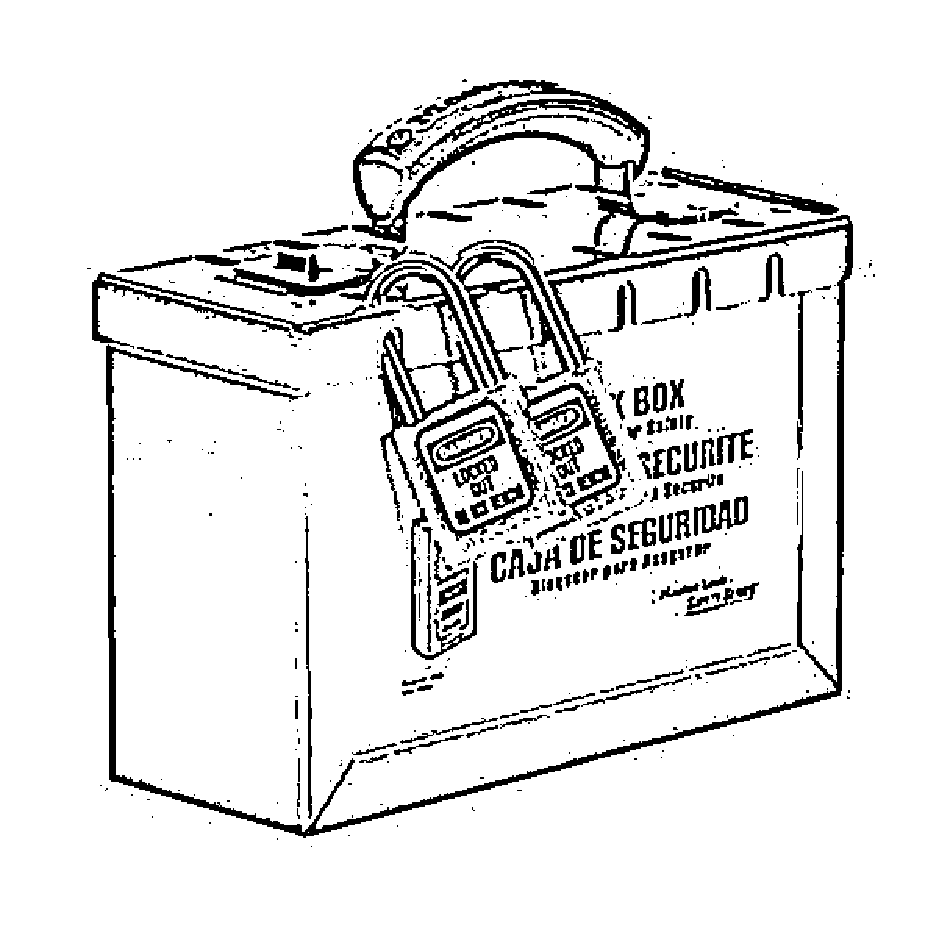
\includegraphics[scale=.18]{box.pdf}
    \end{center}
    \end{stepitemize}
\end{frame}

\begin{frame}{Mathematical solution}
\begin{stepitemize}
\item Alice and Bob agree on a modulus $m$.
\item Alice chooses the secret $a$ with $(a,m)=1$ and chooses her encryption key $e$ such that $(e, \phi(m))=1$
\item Alice sends Bob $a^e \pmod{m}$.
\item Bob chooses his own encryption key $d$ such that $(d, \phi(m))=1$ and then he sends Alice $(a^e)^d$.
\item Now Alice ``unlocks" her lock, that is with $e^{-1}$ being the mult. inv. of $e$ mod $m$, she sends Bob $((a^e)^d)^{e^{-1}}$.
\item Bob finally ``unlocks" his own lock, that is he computes
$(((a^e)^d)^{e^{-1}})^{d^{-1}}$ and finds $a$.
\item The mathematical correctness of this scheme follows from
$a^{k\phi(m)+1} \equiv a \pmod{m}$ by Euler's Congruence.
\end{stepitemize}
\end{frame}

\begin{frame}{A Toy Example}
\begin{stepitemize}
\item Assume $m= 641\cdot 3319=2,127,479.$
\item Then $\phi(m)=640\cdot 3318=2,123,520.$
\item Let $a=1023$, $e=191$, which means $e^{-1} = 1,534,271$ and $d=2987$, which means $d^{-1} = 519,683$
\item[]
\begin{center}
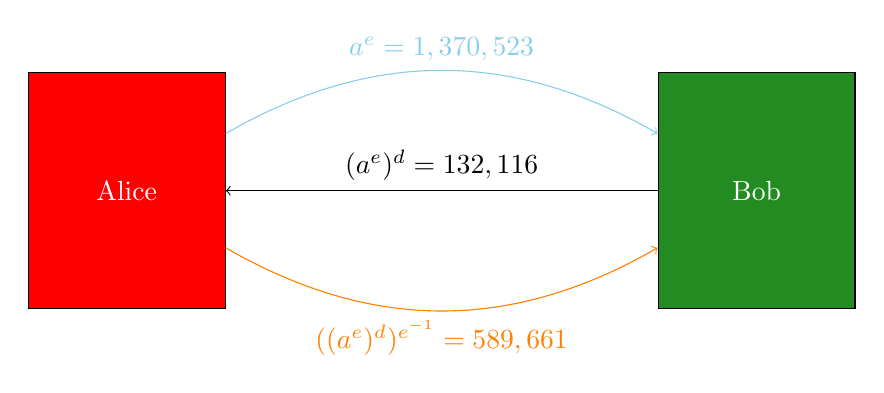
\begin{tikzpicture}
\node[fill=red, text=white, rectangle,draw,  minimum width = 2.5cm,
    minimum height = 3cm] (r1) at (0,0) {Alice};

 \node[fill=ForestGreen, text=white,rectangle,draw,  minimum width = 2.5cm,
    minimum height = 3cm] (r2) at (8,0) {Bob};
\draw[->,bend left, SkyBlue] (r1) edge node[above]{$a^e = 1,370,523$}(r2);
\draw[->] (r2) -- node[above]{$(a^e)^d = 132,116$}(r1);
\draw[->,bend right, orange]  (r1) edge node[below]{$((a^e)^d)^{e^{-1}} = 589,661$}(r2);
\end{tikzpicture}
\end{center}
\item Finally Bob calculates $589661^{519683}$ modulo $2,127,429$ and finds $1023$, which is the original number.
\end{stepitemize}
\end{frame}

\begin{frame}{RSA}
\begin{stepitemize}
    \item One of the first examples of Public Key cryptosystems
    \item Came out in 1978
    \item In this scheme there are two keys. One is called ``the Public Key" and the other called ``the Secret Key".
    \item {\bf Public Key:} For two large primes $p, q$ let $n=pq$. The public key is the ordered pair $(n,e)$ where $(e, \phi(n))=1$.
    \item {\bf Secret Key:} $p, q$ and $d$ such that $d\equiv e^{-1} \pmod{\phi(n)}$.
    \item The security of the scheme depends on the hardness of factorization.
    \item The scheme would be broken if we can find $p, q$ from $n$.
    \end{stepitemize}
    \end{frame}

\begin{frame}{Encryption-Decryption}
\begin{stepitemize}
    \item  One chooses $m$ as the message (a number, such that $(m,n)=1$).
    \item Encryption: $m^e$ modulo $n$.
    \item Decryption: $(m^e)^d$ modulo $n$.
    \item The scheme works since
$$(m^e)^d = m^{1+\phi(m)\cdot k} \equiv m \pmod{n}$$
by Euler's congruence theorem.

\end{stepitemize}

\end{frame}

\begin{frame}{A Toy Example}
\begin{stepitemize}
\item Let $n=641\cdot643 = 412163$.
\item Then we have $\phi(n)=640\cdot 642 = 410880$.
\item Choose $e=1561$.
\item So the public key is the pair $(n,e) = (412163,1561)$.
\item The multiplicative inverse $d$ of $e$ mod $\phi(n)$ is given by $281641$.
\item The secret key is the triple $(p,q,d) = (641, 642,281641)$.
\item If we want to encrypt the message $m=54637$, then we send $m^e \pmod{n}$, which is $362033$.
\item To decrypt, we calculate $362033^{281641}$ modulo $412163$, which turns out to be $54637$, which is the original message.
\end{stepitemize}
\end{frame}

\section{Order of Elements in moduli, Primitive Elements}
\begin{frame}{Order of Elements}
    \begin{stepitemize}
    \item Recall that $a^{\phi(n)} \equiv 1 \pmod{n}$ for $GCD(a,n)=1$
    \item So, for example $2^6\equiv 1 \pmod{7}$
    \item But we also have $2^3\equiv 1 \pmod{7}$.
    \item The order of $a$ modulo $n$, denoted by $ord_n(a)$ is the smallest positive power of $a$ that is equivalent to 1 modulo $n$.
    \item In other words
    $$ord_n(a)=h \Leftrightarrow a^h \equiv 1 \pmod{n}, \:\:\: a^k\not \equiv 1 \pmod{n}, \:\:\:  1\leq k < h.$$
    \item For example, $ord_7(2)=3$ and $ord_7(3)=6$.
    \item The following is a main theorem about orders:
    \item {\bf Theorem}:\\
Suppose $ord_n(a)=h$. Then $a^m\equiv 1 \pmod{n}$ if and only if $h|m$. In particular, $ord_n(a)|\phi(n)$ for all $n>1$ and $a: (a,n)=1$.
    \end{stepitemize}
\end{frame}
\begin{frame}
\begin{stepitemize}
\item As an example let us try to find $ord_{18}(5)$.
\item By the theorem we know $ord_{18}(5)|\phi(18)=6$.
\item So we just need to check $5^2, 5^3$ modulo $18$.
\item $5^2=25 \equiv 7 \pmod{18}$ and so $5^3 \equiv 35 \equiv 17 \pmod{18}$.
\item This shows that $ord_{18}(5)\neq 1, 2$ or $3$, so we must have $ord_{18}(5)=6$.
\end{stepitemize}
\end{frame}

\begin{frame}{Another Important Property}
\begin{stepitemize}
\item The following is another important property of order:
\item {\bf Theorem:}\\
If $ord_n(a)=h$, then $\{1,a,a^2, \dots, a^{h-1}\}$ are all distinct modulo $n$.

\item We have the following immediate corollary:
\item {\bf Corollary:}\\
If $ord_n(a)=\phi(n)$, then $\{1,a, a^2, \dots, a^{\phi(n)-1}\}$ forms a $C.S.R.R.C$ modulo $n$. In other words, we have
$$\{1,a, a^2, \dots, a^{\phi(n)-1}\} \equiv \Z_n^{\times} \pmod{n}.$$

\end{stepitemize}

\end{frame}

\begin{frame}
\begin{stepitemize}
\item As an example we look at powers of $3$ mod $7$:
$$\{3^1, 3^2, 3^3, 3^4, 3^5, 3^6\} \equiv \{3, 2, 6, 4, 5, 1\} \pmod{7}$$
\item Similarly we can look at powers of $2$ modulo $11$:
$$\{2^1, 2^2, 2^3, 2^4, 2^5, 2^6, 2^7, 2^8, 2^9, 2^{10}\} \equiv \{2, 4, 8, 5, 10, 9, 7, 3, 6, 1\} \pmod{11}.$$
\item The following picture visualizes the matching:

\bigskip
\begin{center}
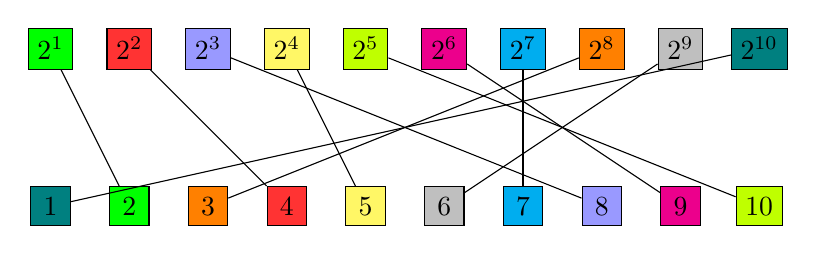
\begin{tikzpicture}
\node[fill=green, text= black, rectangle,draw,  minimum width = 0.5cm,
    minimum height = 0.5cm] (r1) at (0,0) {$2^1$};
\node[fill=red!80, text= black, rectangle,draw,  minimum width = 0.5cm,
    minimum height = 0.5cm] (r2) at (1,0) {$2^2$};
\node[fill=blue!40, text= black,rectangle,draw,  minimum width = 0.5cm,
    minimum height = 0.5cm] (r3) at (2,0) {$2^3$};

\node[fill=yellow!60, text= black, rectangle,draw,  minimum width = 0.5cm,
    minimum height = 0.5cm] (r4) at (3,0) {$2^4$};
\node[fill=lime, text= black, rectangle,draw,  minimum width = 0.5cm,
    minimum height = 0.5cm] (r5) at (4,0) {$2^5$};
\node[fill=magenta, text= black,rectangle,draw,  minimum width = 0.5cm,
    minimum height = 0.5cm] (r6) at (5,0) {$2^6$};
\node[fill=cyan, text= black,rectangle,draw,  minimum width = 0.5cm,
    minimum height = 0.5cm] (r7) at (6,0) {$2^7$};
\node[fill=orange, text= black,rectangle,draw,  minimum width = 0.5cm,
    minimum height = 0.5cm] (r8) at (7,0) {$2^8$};
\node[fill=lightgray, text= black,rectangle,draw,  minimum width = 0.5cm,
    minimum height = 0.5cm] (r9) at (8,0) {$2^9$};
\node[fill=teal, text= black,rectangle,draw,  minimum width = 0.5cm,
    minimum height = 0.5cm] (r10) at (9,0) {$2^{10}$};

\node[fill=teal, text= black,rectangle,draw,  minimum width = 0.5cm,
    minimum height = 0.5cm] (q1) at (0,-2) {$1$};
\node[fill=green, text= black, rectangle,draw,  minimum width = 0.5cm,
    minimum height = 0.5cm] (q2) at (1,-2) {$2$};
\node[fill=orange, text= black,rectangle,draw,  minimum width = 0.5cm,
    minimum height = 0.5cm] (q3) at (2,-2) {$3$};

\node[fill=red!80, text= black, rectangle,draw,  minimum width = 0.5cm,
    minimum height = 0.5cm] (q4) at (3,-2) {$4$};
\node[fill=yellow!60, text= black,rectangle,draw,  minimum width = 0.5cm,
    minimum height = 0.5cm] (q5) at (4,-2) {$5$};
\node[fill=lightgray, text= black,rectangle,draw,  minimum width = 0.5cm,
    minimum height = 0.5cm] (q6) at (5,-2) {$6$};
\node[fill=cyan, text= black,rectangle,draw,  minimum width = 0.5cm,
    minimum height = 0.5cm] (q7) at (6,-2) {$7$};
\node[fill=blue!40, text= black,rectangle,draw,  minimum width = 0.5cm,
    minimum height = 0.5cm] (q8) at (7,-2) {$8$};
\node[fill=magenta, text= black,rectangle,draw,  minimum width = 0.5cm,
    minimum height = 0.5cm] (q9) at (8,-2) {$9$};
\node[fill=lime, text= black,rectangle,draw,  minimum width = 0.5cm,
    minimum height = 0.5cm] (q10) at (9,-2) {$10$};

\draw (r1)--(q2);
\draw (r2)--(q4);
\draw (r3)--(q8);
\draw (r4)--(q5);
\draw (r5)--(q10);
\draw (r6)--(q9);
\draw (r7)--(q7);
\draw (r8)--(q3);
\draw (r9)--(q6);
\draw (r10)--(q1);
\end{tikzpicture}
\end{center}

\end{stepitemize}
\end{frame}
\begin{frame}
\begin{stepitemize}

\item We can find orders of powers using the following result:
\item {\bf Theorem:} \\
If $ord_n(a)=h$, then $ord_n(a^k) = \frac{h}{GCD(h,k)}$.

\item For example $ord_{11}(2)=10$, which means $ord_{11}(4)=5$ and $ord_{11}(8)=10/(3,10)=10.$

\item The following corollary immediately follows:
\item {Corollary:}
If $ord_{n}(a)=h$, then $ord_n(a^k)=h$ if and only if $GCD(h,k)=1$.
\end{stepitemize}
\end{frame}

\begin{frame}{Primitive Roots}
\begin{stepitemize}
    \item A primitive root is a special element that generates the whole CSRRC modulo $n$.
    \item So a primitive root $a$ modulo $n$ has $ord_n(a)=\phi(n)$.
    \item It has the maximal possible order.
    \item So $3$ is a primitive root modulo $7$ while $2$ is not a primitive root modulo $7$.
    \item Two main questions regarding primitive elements:
\begin{enumerate}
    \item For which $n>1$, does there exist a primitive element modulo $n$?
    \item If there is a primitive element modulo $n$, how many primitive elements are there?
\end{enumerate}
\end{stepitemize}
\end{frame}

\begin{frame}
\begin{stepitemize}
    \item  $\phi(12)=4$ and the numbers relatively prime to $12$ are $1, 5, 7$ and $11$, but
$$1^2\equiv 5^2\equiv 7^2\equiv 11^2 \equiv 1 \pmod{12}$$ so there are no primitive elements modulo $12$.
\item Similarly $1^2 \equiv 7^2 \equiv 9^2 \equiv 15^2 \equiv 1 \pmod{16}$, whereas $3^4 \equiv5^4\equiv 11^4 \equiv 13^4 \equiv 1 \pmod{16}$. Since $\phi(16)=8$, there are no primitive elements modulo $16$.
\item We can eliminate more numbers from the following results:
\item {\bf Theorem:} \\
Let $m\geq 1$ be any integer and let $a$ be any odd integer. Then we have
$$a^{2^m} \equiv 1 \pmod{2^{m+2}}.$$
\item {\bf Corollary:} \\
Since $\phi(2^{m+2})=2^{m+1}$, the previous theorem shows that there is no primitive element modulo $2^{m}$ for $m\geq 3$.
\end{stepitemize}

\end{frame}

\begin{frame}
    \begin{stepitemize}
    \item The following theorem helps eliminate a much bigger set of numbers:
\item {\bf Theorem:}\\
If $n=mk$, where $m,k>2$ and $GCD(m,k)=1$, then there is no primitive element modulo $n$.
\item As a corollary to the previous theorems we have the following result:
\item {\bf Corollary:}\\
If there is a primitive element modulo $n$ then $n$ must be $2$, $4$, $p^k$ or $2p^k$, where $p$ is an odd prime.
\item It turns out that this result is actually two sided:
\item {\bf Theorem:}\\
There is a primitive element modulo $n$ if and only if $n$ is 2, 4, $p^k$ or $2p^k$, where $p$ is an odd prime.
    \end{stepitemize}

\end{frame}
\begin{frame}{Number of Primitive roots}
    \begin{stepitemize}
    \item Recall that if $a$ is a primitive element modulo $n$, then
$$\{1, a, a^2, \dots, a^{\phi(n)-1}\} \equiv \Z_n^{\times} \pmod{n}.$$
\item Also recall that if $ord_n(a)=h$ then $ord_n(a^k)=\frac{h}{(k,h)}$.
\item Thus if there is a primitive element modulo $n$, then $a^k$ is also primitive root whenever $(k,\phi(n))=1$.
\item But we know what this number is:
\item {\bf Theorem:} \\
If there is a primitive element modulo $n$, then there are exactly $\phi(\phi(n))$ primitive elements modulo $n$.
\item For example, we know $2$ is a primitive root mod $11$. Thus there are $\phi(\phi(11))=\phi(10)=4$ primitive roots mod $11$, and they are given by $2, 2^3=8, 2^7=7, 2^9=6$.
    \end{stepitemize}
\end{frame}
\begin{frame}
\centerline{\color{ForestGreen}\bf{\Large THANK YOU!!!}}

\end{frame}

\end{document}
